\documentclass[10pt,a4paper]{article}
\usepackage{fontspec,amsmath,amssymb,amsthm,mathtools,graphicx,bm,bbm,stmaryrd,nicefrac}
\usepackage[margin=22mm]{geometry}
\usepackage[bookmarks=false]{hyperref}
\setlength{\emergencystretch}{3em}
\title{Counting-measure zero for infinitely often time-bounded compressible prefixes}
\author{John M. Hitchcock, Adewale Sekoni, Hadi Shafei}
\date{doi:10.4230/LIPIcs.CCC.2025.20; CC BY 4.0}
\begin{document}
\maketitle
\noindent\textit{Editorial note.} Editable TeX converted from the official CC BY HTML prose and math alttext. Original official PDF/HTML retained. Only the specified claim counts; all author context and available source-local supporting proofs are included.\par\medskip
\noindent\textit{Allowed standard prerequisites (editorial).}\begin{itemize}
\item Standard finite probability and the cited sampler/extractor or multicalibration results. Definitions and all source-local support proofs are retained; cited established results are used as the authors state.
\end{itemize}\medskip


\par\medskip\noindent\textbf{
1 Introduction}\par




Resource-bounded measures and dimensions [48, 49, 50, 52, 7] are fundamental tools for analyzing complexity classes, offering refined ways to understand the power and limitations of different computational resources [51, 33, 56, 3].
Traditional approaches based on real-valued martingales provide insights into classes like $\mathsf{P}$, $\mathsf{NP}$, $\mathsf{PSPACE}$, and $\mathsf{EXP}$ but they leave gaps when it comes to many intermediate complexity classes. This paper introduces counting martingales, which offer a new perspective on these intermediate classes by utilizing functions from counting complexity classes.\par




Our main contributions are:\par


\begin{enumerate}


\item[] 
1. 


Counting Martingales and Counting Measures and Dimensions: We introduce counting martingales, which generalize traditional martingales by incorporating functions from ${\mathsf{\#}\mathsf{P}}$, $\mathsf{SpanP}$, and $\mathsf{GapP}$, creating intermediate complexity measures and dimensions. We define ${\mathsf{\#}\mathsf{P}}$-measure, $\mathsf{SpanP}$-measure, and $\mathsf{GapP}$-measure as intermediate measures between $\mathsf{P}$-measure and $\mathsf{PSPACE}$-measure, allowing finer analysis of complexity classes.\par





\item[] 
2. 


Applications to Circuit Complexity: Using these new measures, we provide novel results on nonuniform complexity and the Shannon-Lupanov bound. Shannon’s $(1-\epsilon)\frac{2^{n}}{n}$ lower bound (1949) was improved by Lutz (1992) who showed that for any $\alpha<1$, almost all problems require circuits of size $\frac{2^{n}}{n}\!\left(1+\frac{\alpha\log n}{n}\right)$. We improve this result further by extending it to $\mathsf{SpanP}$-measure. In our proof, we construct a counting martingale using a connection through the Minimum Circuit Size Problem ($\mathsf{MCSP}$). Moreover, we study classical and quantum circuit complexity classes using ${\mathsf{\#}\mathsf{P}}$-dimension and $\mathsf{GapP}$-dimension, respectively.\par





\end{enumerate}




The standard definitions of resource-bounded measure use martingales that are real-valued functions computable within deterministic time and space resource bounds [50].
In this paper, we use the counting complexity classes ${\mathsf{\#}\mathsf{P}}$ [76], $\mathsf{SpanP}$ [41], and $\mathsf{GapP}$ [18, 45]
to introduce the concept of \emph{counting martingales} and define \emph{counting measures} and \emph{counting dimensions} that are intermediate in power between the previous time- and space-bounded measures and dimensions. A ${\mathsf{\#}\mathsf{P}}$ function counts the number of accepting paths of a probabilistic Turing machine ($\mathsf{PTM}$), while a $\mathsf{SpanP}$ function counts the number of different outputs of a $\mathsf{PTM}$. Every ${\mathsf{\#}\mathsf{P}}$ function is also a $\mathsf{SpanP}$ function, and the classes are equal if and only if $\mathsf{UP}=\mathsf{NP}$ [41].
A $\mathsf{GapP}$ function counts the difference between the number of accepting paths and the number of rejecting paths of a $\mathsf{PTM}$ [18, 45]. For more background on counting complexity, we refer to the surveys [69, 21].\par




A martingale is
a function $d:\{0,1\}^{*}\to[0,\infty)$ such that\par


\[\begin{gathered}
d(w)=\frac{d(w0)+d(w1)}{2}
\end{gathered}\]


for all $w\in\{0,1\}^{*}$.
We view a martingale as acting on Cantor Space $\mathsf{C}=\{0,1\}^{\infty}$ (the infinite binary tree). The value at any node is the average of the values below it. By induction, the value at any node is also the average of the values at any level of the subtree below the node:\par


\[\begin{gathered}
d(w)=\frac{1}{2^{n}}\sum_{x\in\{0,1\}^{n}}d(wx).
\end{gathered}\]


A martingale starts with a finite amount $d(\lambda)$ at the root. We may assume $d(\lambda)=1$ without loss of generality.\par




Intuitively, because the average value of a martingale across $\{0,1\}^{n}$ is $d(\lambda)=1$, a martingale is unable to obtain “large” values on “many” sequences. This intuition is formalized into characterizations of
Lebesgue measure [44] and Hausdorff dimension [27] using martingales. A class $X\subseteq\mathsf{C}$ has measure 0 if and only if there is a martingale that attains unbounded values on all elements of $X$ [78]. A class $X\subseteq\mathsf{C}$ has Hausdorff dimension $s$ if $2^{(1-s)n}$ is the optimal growth rate of martingales on $X$ [52].\par




Resource-bounded measure and dimension come from restricting these characterizations to martingales computable within some complexity class [50, 52, 7]. The most used resource bounds are polynomial-time $(\mathsf{P})$ and polynomial-space $(\mathsf{PSPACE})$.
Generally, it is much easier to construct $\mathsf{PSPACE}$-martingales than it is $\mathsf{P}$-martingales [38, 32]. For more background on resource-bounded measure and dimension we refer to the surveys [51, 56, 3, 33, 74].\par




\par\medskip\noindent\textbf{
1.1 Counting Martingales}\par



\par\noindent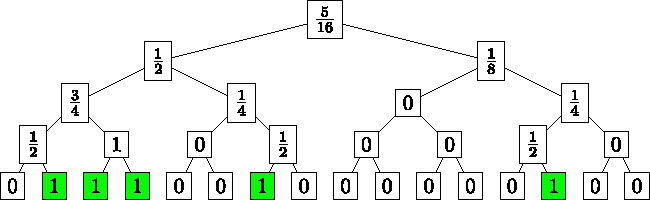
\includegraphics[width=\linewidth,height=0.78\textheight,keepaspectratio]{ccc2025-20-svg-01.pdf}\par

Figure 1.1: Cover Martingale Construction (Construction 4.1).



Our conceptual contribution is the introduction of \emph{counting martingales}, which provide intermediate measure and dimension notions between $\mathsf{P}$ and $\mathsf{PSPACE}$ by using functions from counting complexity classes to define martingales. Many martingale constructions in complexity theory are expressed naturally as counting martingales.\par




For example, a standard technique for constructing a martingale is betting on a
cover (see Figure 1.1) [51, 3].
Given a set $A\subseteq\{0,1\}^{*}$ and $n\geq 1$, we choose $x\in\{0,1\}^{n}$ uniformly at random and define a martingale
$d_{A}$ by\par


\[\begin{gathered}
d_{A}(w)=\underset{x\in\{0,1\}^{n}}{\mathsf{Pr}}\left[x\in A\mid w\sqsubseteq x\right]=\frac{|\{x\in A\cap\{0,1\}^{n}\mid w\sqsubseteq x\}|}{2^{n-|w|}}
\end{gathered}\]


for all $w\in\{0,1\}^{\leq n}$. Strings of longer length have the value of their length-$n$ prefix. If we can construct an infinite family of such martingales that cover a class and the sum of their initial values converges, the Borel-Cantelli lemma applies to show the class has measure 0 [17].\par




A key difference between space-bounded measure and time-bounded
measure is that a space-bounded martingale can enumerate a covering,
whereas a time-bounded martingale does not have time to do this.
The complexity of computing $d_{A}$ depends on the complexity of $A$ and the enumeration bottleneck.
Suppose that $A\in\mathsf{P}$.
Naively computing $d_{A}$ would involve an
enumeration of $A$, requiring polynomial space.
Computing $d_{A}$ in polynomial time would only be possible if we have some special
structure in $A$. For example, if $A$ is $\mathsf{P}$-rankable [2], then $d_{A}$ is
polynomial-time computable [35]. It is also possible
to approximately compute $d_{A}$ using an oracle from the
polynomial-time hierarchy [73, 59, 35].\par




However, the numerator in the definition of $d_{A}$ is in general a ${\mathsf{\#}\mathsf{P}}$
function if $A\in\mathsf{P}$. This is because we can use a $\mathsf{PTM}$ (Probabilistic Turing Machine) to count how many extensions of a string are in the cover. We call this a ${\mathsf{\#}\mathsf{P}}$ martingale. In general, a martingale is a ${\mathsf{\#}\mathsf{P}}$ martingale if it can be approximated by the
ratio of a ${\mathsf{\#}\mathsf{P}}$ function and a polynomial-time function.\par




The case when the cover $A\in\mathsf{NP}$ is also interesting, for example when $A$ is the Minimum Circuit Size Problem ($\mathsf{MCSP}$). Then the numerator is a $\mathsf{SpanP}$ function. While a ${\mathsf{\#}\mathsf{P}}$ function counts the number of acceptings paths of a $\mathsf{PTM}$, a $\mathsf{SpanP}$ function counts the number of distinct values output by a $\mathsf{PTM}$. A martingale of this form is a $\mathsf{SpanP}$-martingale.\par




When we use a $\mathsf{GapP}$ function for the numerator of a martingale, we call it a $\mathsf{GapP}$-martingale. We will show that $\mathsf{GapP}$-martingales are capable of measuring quantum complexity classes. Until now, quantum complexity has not been addressed by resource-bounded measure.\par




We call ${\mathsf{\#}\mathsf{P}}$-martingales, $\mathsf{SpanP}$-martingales, and $\mathsf{GapP}$-martingales \emph{counting martingales}.
Definition 3.1 contains the formal definitions of counting martingales.\par





\par\medskip\noindent\textbf{
1.2 Counting Measures and Counting Dimensions}\par




A class $X$ has ${\mathsf{\#}\mathsf{P}}$-measure 0, written $\mu_{{\mathsf{\#}\mathsf{P}}}(X)=0$,
if there is a ${\mathsf{\#}\mathsf{P}}$-martingale that succeeds on $X$.
Analogously, a class $X$ has $\mathsf{SpanP}$-measure 0, written $\mu_{\mathsf{SpanP}}(X)=0$,
if there is a $\mathsf{SpanP}$-martingale that succeeds on $X$. Furthermore, a class $X$ has
$\mathsf{GapP}$-measure 0, written $\mu_{\mathsf{GapP}}(X)=0$, if there is a $\mathsf{GapP}$-martingale that succeeds on $X$.
These \emph{counting measures} are
intermediate between $\mathsf{P}$-measure and $\mathsf{PSPACE}$-measure:
for every class $X\subseteq\mathsf{C}$,\par


\[\begin{gathered}
\begin{array}[]{ccccccc}\mu_{\mathsf{P}}(X)=0&\Rightarrow&\mu_{{\mathsf{\#}\mathsf{P}}}(X)=0&\Rightarrow&\mu_{\mathsf{GapP}}(X)=0\\
&&\Downarrow&&\Downarrow\\
&&\mu_{\mathsf{SpanP}}(X)=0&\Rightarrow&\mu_{\mathsf{PSPACE}}(X)=0&\Rightarrow&\mu(X)=0.\end{array}
\end{gathered}\]


We do not know of any relationship between $\mu_{\mathsf{SpanP}}$ and $\mu_{\mathsf{GapP}}$.
An individual problem $B$ is $\Delta$\emph{-random} if no $\Delta$-martingale succeeds on $B$.
We show that $\mathsf{UP}$ problems are not ${\mathsf{\#}\mathsf{P}}$-random and $\mathsf{NP}$ problems are not $\mathsf{SpanP}$-random. This is interesting in comparison to the result that $\mathsf{SpanP}={\mathsf{\#}\mathsf{P}}$ if and only if $\mathsf{NP}=\mathsf{UP}$ [41].
When we have a proposition that is known in $\mathsf{PSPACE}$-measure, but open in
$\mathsf{P}$-measure, we can investigate it in ${\mathsf{\#}\mathsf{P}}$-measure, $\mathsf{SpanP}$-measure, or $\mathsf{GapP}$-measure.\par




We also introduce \emph{counting dimensions}, ${\mathsf{\#}\mathsf{P}}$-dimension, $\mathsf{SpanP}$-dimension, and $\mathsf{GapP}$-dimension, which analogously fall between $\mathsf{P}$-dimension and $\mathsf{PSPACE}$-dimension. For all $X\subseteq\mathsf{C}$,\par


\[\begin{gathered}
\begin{array}[]{ccccccc}0\leq{\mathsf{dim}}_{\mathsf{H}}(X)&\leq&{\mathsf{dim}}_{\mathsf{PSPACE}}(X)&\leq&{\mathsf{dim}}_{\mathsf{GapP}}(X)\\
&&\mathrel{\raisebox{4.30554pt}{\rotatebox{270.0}{$\leq$}}}&&\mathrel{\raisebox{4.30554pt}{\rotatebox{270.0}{$\leq$}}}\\
&&{\mathsf{dim}}_{\mathsf{SpanP}}(X)&\leq&{\mathsf{dim}}_{\mathsf{\#}\mathsf{P}}(X)&\leq&{\mathsf{dim}}_{\mathsf{P}}(X)\leq 1.\end{array}
\end{gathered}\]


We do not know of any relationship between ${\mathsf{dim}}_{\mathsf{SpanP}}$ and ${\mathsf{dim}}_{\mathsf{GapP}}$.
We work out the basic properties of counting measures and dimensions in Section 3.\par





\par\medskip\noindent\textbf{
1.3 Our Techniques}\par




Many martingale constructions in complexity theory are expressed naturally as counting martingales.
These and other martingale constructions we need in this paper follow similar patterns.
In Section 4 we present a few martingale constructions in a unified framework.\par



\par\noindent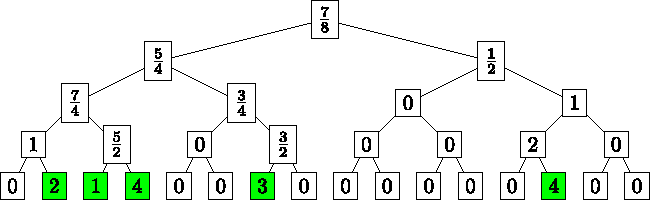
\includegraphics[width=\linewidth,height=0.78\textheight,keepaspectratio]{ccc2025-20-svg-02.pdf}\par

Figure 1.2: Conditional Expectation Martingale Construction (Construction 4.3).



\begin{enumerate}


\item[] 
1. 


\textbf{Cover Martingale.} The Cover Martingale construction utilizes a covering set $A$ and defines the martingale based on the conditional probability that an extension of the current string belongs to $A$. If $A\in\mathsf{UP}$, this construction produces a ${\mathsf{\#}\mathsf{P}}$-martingale; if $A\in\mathsf{NP}$, it results in a $\mathsf{SpanP}$-martingale. If $A$ is in the counting complexity class $\mathsf{SPP}$, then this generates a $\mathsf{GapP}$-martingale. The class $\mathsf{SPP}$ consists of all languages $L$ for which there exists a $\mathsf{GapP}$ function $f$ such that if $x\in L$ then $f(x)=1$, and $f(x)=0$ otherwise [18]. This approach is effective for capturing known martingale constructions in the literature, particularly in scenarios where membership within a subset can be determined with unique or nondeterministic witnesses. For further details, refer to Figure 1.1 and Construction 4.1.\par





\item[] 
2. 


\textbf{Conditional Expectation Martingale.} This martingale generalizes the Cover Martingale by using a counting function $f(x)$ as a random variable and taking its conditional expectation given the current prefix $w$. This construction is adaptable to functions within ${\mathsf{\#}\mathsf{P}}$, $\mathsf{SpanP}$ and $\mathsf{GapP}$, making it effective for applications that require combining information from extensions of a given string. The Conditional Expectation Martingale averages the values of $f$ over all extensions, providing a flexible tool. See Figure 1.2 and Construction 4.3 for an example and technical details.\par





\item[] 
3. 


\textbf{Subset Martingale.} This martingale is designed to succeed on all infinite subsets of a language $B$. If $B\in\mathsf{UP}$, it produces a ${\mathsf{\#}\mathsf{P}}$-martingale, and if $B\in\mathsf{NP}$, it yields a $\mathsf{SpanP}$-martingale. If $B\in\mathsf{SPP}$, then this is a $\mathsf{GapP}$-martingale. Unlike deterministic martingales that can focus directly on a language, the Subset Martingale is unique in its ability to succeed across all subsets of a language. This property allows us to conclude that ${\mathsf{\#}\mathsf{P}}$-random languages are not in $\mathsf{UP}$, $\mathsf{SpanP}$-random languages are not in $\mathsf{NP}$, and $\mathsf{GapP}$-random languages are not in $\mathsf{SPP}$. See Figure 4.1 for an example and Construction 4.5 for a formal definition.\par





\item[] 
4. 


\textbf{Acceptance Probability Martingale.}
We also show that betting according to the acceptance probabilites of a $\mathsf{PTM}$ or $\mathsf{QTM}$ (quantum Turing machine) yields a counting martingale. Using this, we show that $\mathsf{BPP}$ has ${\mathsf{\#}\mathsf{P}}$-dimension 0 and $\mathsf{BQP}$ has $\mathsf{GapP}$-dimension 0. See Figure 4.2 for an example and Construction 4.9 for a formal definition.\par





\item[] 
5. 


\textbf{Bi-Immunity Martingale.} Mayordomo [59] showed $\mathsf{P}$-random languages are $\mathsf{E}$-bi-immune and $\mathsf{PSPACE}$-random languages are $\mathsf{ESPACE}$-bi-immune using a construction that we call a bi-immunity martingale.
This construction is designed to succeed on all supersets of an infinite language. We show that this construction works as counting martingales to show ${\mathsf{\#}\mathsf{P}}$-random languages are $\mathsf{UP}\cap\mathsf{co}\mathsf{UP}$-bi-immune, $\mathsf{SpanP}$-random languages are $\mathsf{NP}\cap\mathsf{co}\mathsf{NP}$-bi-immune, and $\mathsf{GapP}$-random languages are $\mathsf{SPP}$-bi-immune.\par





\end{enumerate}




\par\medskip\noindent\textbf{Entropy Rates.}\par




Hitchcock and Vinodchandran [35] showed a covering notion called the $\mathsf{NP}$-entropy rate is an upper bound for ${\Delta^{\mathsf{P}}_{3}}$-dimension, where ${\Delta^{\mathsf{P}}_{3}}=\mathsf{P}^{{\Sigma^{\mathsf{P}}_{2}}}$. In Section 5.1, we extend this by showing that $\mathsf{SpanP}$-dimension lies between ${\Delta^{\mathsf{P}}_{3}}$-dimension and the $\mathsf{NP}$-entropy rate. Informally, for a complexity class ${\cal C}$ and $X\subseteq\mathsf{C}$, the ${\cal C}$-entropy rate of $X$ is the infimum $s$ for which all elements of $X$ can be covered infinitely often by a language $A\in{\cal C}$ that has $\frac{\log|A_{=n}|}{n}\leq s$ for all sufficiently large $n$. Intuitively, this corresponds to using $A$ as an implicit code, where it takes $\log|A_{=n}|$ bits to specify a member of $A_{=n}$.\par





\par\medskip\noindent\textbf{Kolmogorov Complexity.}\par




In Section 5.2, we connect
${\mathsf{\#}\mathsf{P}}$-measure and ${\mathsf{\#}\mathsf{P}}$-dimension to Kolmogorov complexity. For a time bound $t(n)$, $K^{t}(x)$ is the length of the shortest program that prints $x$ in $t(|x|)$ time on a universal Turing machine. In particular, we extend a result from Lutz [50] and show that $\{S\mid(\exists^{\infty}n)K^{p}(S\negthinspace\upharpoonright\negthinspace n)<n-f(n)\}$ has ${\mathsf{\#}\mathsf{P}}$-measure 0, where $p$ is a polynomial, and $\sum_{n=0}^{\infty}2^{-f(n)}$ is a $\mathsf{P}$-convergent series. In other words, we prove that if $S$ is ${\mathsf{\#}\mathsf{P}}$-random, then $K^{p}(S\negthinspace\upharpoonright\negthinspace n)\geq n-f(n)$ almost everywhere.\par






\par\medskip\noindent\textbf{
1.4 Our Results}\par




In Section 6 we study the measure and dimension of classical and quantum circuit complexity classes.
Shannon [71] showed that almost all Boolean functions on $n$ input bits require $(1-\epsilon)\frac{2^{n}}{n}$-size circuits.
Lutz [50] strengthened this in two ways,
showing that the larger circuit complexity class\par


\[\begin{gathered}
X_{\alpha}=\mathsf{SIZE}^{\mathsf{i.o.}}\!\!\left(\frac{2^{n}}{n}\left(1+\frac{\alpha\log n}{n}\right)\right)
\end{gathered}\]


has $\mathsf{PSPACE}$-measure 0 for all $\alpha<1$.
Frandsen and Miltersen [24] strengthened the original upper bound of Lupanov [47] to show that Lutz’s bound is nearly tight: $X_{\alpha}$ contains all problems when $\alpha>3$.\par




We improve Lutz’s result to show that $\mu_{\mathsf{SpanP}}(X_{\alpha})=0$. Lutz’s proof extensively reuses polynomial space to consider only \emph{novel} circuits, that compute a different function than any previously considered circuit. This proof does not adapt easily to our setting. In Section 5, we introduce a measure notion called ${{\cal M}_{\mathsf{NP}}}$ that bridges the gap between
$\mu_{\mathsf{PSPACE}}$ and $\mu_{\mathsf{SpanP}}$ by utilitizing the Minimum Circuit Size Problem ($\mathsf{MCSP}$) [39], allowing the construction of a counting martingale.
As a corollary, we conclude that
$X_{\alpha}$ has measure 0 in the third level
$\Delta^{\mathsf{E}}_{3}=\mathsf{E}^{\Sigma^{\mathsf{P}}_{2}}$ of the exponential-time hierarchy. While it was previously known how to construct a problem in $\Delta^{\mathsf{E}}_{3}$ with maximum circuit-size complexity [64], our result says most problems in $\Delta^{\mathsf{E}}_{3}$ have nearly maximal circuit-size complexity.\par




Li [46], building on work of Korten [42] and Chen, Hirahara, and Ren [14], showed the first exponential-size circuit lower bound within the second level of the exponential-time hierarchy, that the symmetric alternation class $S^{\mathsf{E}}_{2}\not\subseteq\mathsf{SIZE}^{\mathsf{i.o.}}\!\!(\frac{2^{n}}{n}).$ We note that Li’s proof extends to show
$S^{\mathsf{E}}_{2}\not\subseteq\mathsf{SIZE}^{\mathsf{i.o.}}\!\!\left(\frac{2^{n}}{n}\!\left(1+\frac{\alpha\log n}{n}\right)\right)$.
Under suitable derandomization assumptions (see Derandomization Hypothesis 2.7), our $\Delta^{\mathsf{E}}_{3}$ result improves by one level in the exponential hierarchy, showing $X_{\alpha}$ has measure 0 in
$\Delta^{\mathsf{E}}_{2}=\mathsf{E}^{\mathsf{NP}}$.\par




We also improve previous dimension results on circuit-size complexity [52, 35] and density of hard sets [55, 57, 25, 31].
Additionally, we use $\mathsf{GapP}$-martingales to apply our counting measure framework to analyze quantum circuit complexity. We show that the quantum circuit-size class $\mathsf{BQSIZE}\left(o\left(\frac{2^{n}}{n}\right)\right)$ has $\mathsf{GapP}$-dimension 0.
We also show that the class of
problems that ${\mathsf{P}/\mathsf{poly}}$-Turing
reduce to subexponentially dense sets has
${\mathsf{\#}\mathsf{P}}$-measure 0.
See Figure 1.3 for a summary of our results.
We anticipate many further applications of counting measures to refine results where the $\mathsf{PSPACE}$-measure is known and the $\mathsf{P}$-measure is unknown. We discuss some of these directions in Section 7.\par







$\mathsf{SIZE}^{\mathsf{i.o.}}\!\!\left(\frac{2^{n}}{n}\!\left(1+\frac{\alpha\log n}{n}\right)\right)$ 

${{\cal M}_{\mathsf{NP}}}$-measure 0 
Theorem 6.1
 
\par




$\mathsf{SIZE}^{\mathsf{i.o.}}\!\!\left(\frac{2^{n}}{n}\!\left(1+\frac{\alpha\log n}{n}\right)\right)$ 

$\mathsf{SpanP}$-measure 0 
Corollary 6.2
 
\par


$\mathsf{SIZE}^{\mathsf{i.o.}}\!\!\left(\frac{2^{n}}{n}\!\left(1+\frac{\alpha\log n}{n}\right)\right)$ 

${\Delta^{\mathsf{P}}_{3}}$-measure 0 
Corollary 6.3
 
\par


$\mathsf{SIZE}\!\left(\alpha\frac{2^{n}}{n}\right)$ 

${\mathsf{\#}\mathsf{P}}$-dimension $\alpha$
 
Theorem 6.5
 
\par


${\mathsf{P}/\mathsf{poly}}$ 

${\mathsf{\#}\mathsf{P}}$-dimension 0 
Corollary 6.6
 
\par


$\mathsf{SIZE}^{\mathsf{i.o.}}\!\!\left(\alpha\frac{2^{n}}{n}\right)$ 

${\mathsf{\#}\mathsf{P}}$-dimension $\frac{1+\alpha}{2}$
 
Theorem 6.7
 
\par


$\mathsf{BQSIZE}\left(o\left(\frac{2^{n}}{n}\right)\right)$ 

$\mathsf{GapP}$-dimension 0 
Theorem 6.10
 
\par


$({\mathsf{P}/\mathsf{poly}})_{\mathsf{T}}(\mathsf{DENSE}^{c})$ 

${\mathsf{\#}\mathsf{P}}$-dimension 0 
Corollary 6.12
 
\par




Figure 1.3: Summary of New Measure and Dimension Results.




\par\medskip\noindent\textbf{
1.5 Organization}\par




This paper is organized as follows. Section 2 covers preliminaries. Section 3 introduces counting martingales, counting measures, and counting dimensions. In Section 4, we detail the constructions for counting martingales. Section 5 presents our tools on entropy rates and Kolmogorov complexity. Our primary applications on circuit complexity are presented in Section 6. Finally, Section 7 provides concluding remarks and furture directions.\par






\par\medskip\noindent\textbf{
2 Preliminaries}\par




The set of all finite binary strings is $\{0,1\}^{*}$. The empty string
is denoted by $\lambda$. We use the standard enumeration of binary
strings $s_{0}=\lambda,s_{1}=0,s_{2}=1,s_{3}=00,\ldots$. For two
strings $x,y\in\{0,1\}^{*}$, we say $x\leq y$ if $x$ precedes $y$ in
the standard enumeration and $x<y$ if $x$ precedes $y$ and is not
equal to $y$. Given two strings $x$ and $y$, we denote by $[x,y]$ the set of all strings $z$ such that $x\leq z\leq y$. Other types of intervals are defined similarly.
We write $x-1$ for the predecessor
of $x$ in the standard enumeration. We use the notation $x\sqsubseteq y$ to say that
$x$ is a prefix of $y$. The length of a string $x\in\{0,1\}^{*}$ is
denoted by $|x|$.\par




All \emph{languages} (decision problems) in this paper are encoded as
subsets of $\{0,1\}^{*}$. For a language $A\subseteq\{0,1\}^{*}$, we
define $A_{\leq n}=A\cap\{0,1\}^{\leq n}$ and $A_{=n}=A\cap\{0,1\}^{n}$.\par




The \emph{Cantor space} of all infinite binary sequences is $\mathsf{C}$. We
routinely identify a language $A\subseteq\{0,1\}^{*}$ with the element of Cantor space that is $A$’s characteristic sequence according to the
standard enumeration of binary strings. In this way, each complexity
class is identified with a subset of Cantor space. We write $A\negthinspace\upharpoonright\negthinspace n$ for the $n$-bit prefix of the characteristic sequence of $A$, and
$A[n]$ for the $n^{\mathrm{th}}$-bit of its characteristic sequence.
We use $\log$ for the base 2 logarithm.\par




Our definitions of most complexity classes are standard. For any function $s:\mathbb{N}\to\mathbb{N}$, $\mathsf{SIZE}\!(s(n))$ is the class of all
languages $A$ where for all sufficiently large $n$, $A_{=n}$ can be decided
by a circuit with no more than $s(n)$ gates. We write $\mathsf{SIZE}^{\mathsf{i.o.}}\!\!(s(n))$ for the class of all $A$ where $A_{=n}$ has an $s(n)$-size circuit for infinitely many $n$.\par




Lutz used martingales to define resource-bounded measure
[50] and dimension [52].
We review the basic definitions. More background is
available in the survey papers
[51, 62, 54, 33, 3, 56].\par



% SOURCE-ID S2.Thmtheorem1


\par\medskip\noindent\textbf{
\textbf{Definition 2.1}\textbf{ }(Martingale)\textbf{.}
}\par



\emph{A martingale is a function $d:\{0,1\}^{*}\to[0,\infty)$ such
that for all $w\in\{0,1\}^{*}$,}\par


\[\begin{gathered}
d(w)=\frac{d(w0)+d(w1)}{2}.
\end{gathered}\]


\emph{If we relax the equality to an inequality $(\geq)$ in the above equation, we call
$d$ a supermartingale.}\par



% END-SOURCE-ID S2.Thmtheorem1


% SOURCE-ID S2.Thmtheorem2


\par\medskip\noindent\textbf{
\textbf{Definition 2.2}\textbf{ }(Martingale Success)\textbf{.}
}\par



\emph{Let $d$ be a supermartingale or martingale.}\par


\begin{enumerate}


\item[] 
1. 


\emph{We say }$d$\emph{ }succeeds on\emph{ a sequence }$A\in\mathsf{C}$\emph{ if }$\limsup\limits_{n\to\infty}d(A\negthinspace\upharpoonright\negthinspace n)=\infty$\emph{.}\par





\item[] 
2. 


\emph{The }success set\emph{ }$S^{\infty}[d]$\emph{ is the class of sequences that }$d$\emph{ succeeds on.}\par





\item[] 
3. 


\emph{The }unitary success set\emph{ of }$d$\emph{ is the set
}$S^{1}[d]=\{A\in\mathsf{C}\mid(\exists n)\ d(A\negthinspace\upharpoonright\negthinspace n)\geq 1\}.$\emph{}\par





\item[] 
4. 


\emph{For }$s>0$\emph{, we say }$d$\emph{ }$s$-succeeds on\emph{ }$A$\emph{ if }$(\exists^{\infty}n)\ d(S\negthinspace\upharpoonright\negthinspace n)\geq 2^{(1-s)n}$\emph{.}\par





\item[] 
5. 


\emph{We say }$d$\emph{ }$0$-succeeds on\emph{ }$A$\emph{ if }$d$\emph{ }$s$\emph{-succeeds on }$A$\emph{ for all }$s>0$\emph{.}\par





\end{enumerate}



% END-SOURCE-ID S2.Thmtheorem2



In the following definition $\Delta$ can be any of the time or space resource bounds including $\mathsf{P}$, ${\mathsf{P}_{\thinspace\negthinspace{}_{2}}}=\mathsf{QP}$, $\mathsf{PSPACE}$ considered by Lutz [50] and their relativizations including ${\Delta^{\mathsf{P}}_{2}}=\mathsf{P}^{\mathsf{NP}}$, ${\Delta^{\mathsf{P}}_{3}}=\mathsf{P}^{\Sigma^{\mathsf{P}}_{2}}$ [60, 35].\par



% SOURCE-ID S2.Thmtheorem3


\par\medskip\noindent\textbf{
\textbf{Definition 2.3}\textbf{ }(Resource-Bounded Measure and Dimension)\textbf{.}
}\par



\emph{Let $\Delta$ be a resource bound and let $X\subseteq\mathsf{C}$.}\par


\begin{enumerate}


\item[] 
1. 


$X$\emph{ has }$\Delta$-measure 0\emph{, and we write }$\mu_{\Delta}(X)=0$\emph{, if there is a }$\Delta$\emph{-computable martingale }$d$\emph{ with }$X\subseteq S^{\infty}[d]$\emph{.}\par





\item[] 
2. 


$X$\emph{ has }$\Delta$-measure 1\emph{, and we write }$\mu_{\Delta}(X)=1$\emph{, if }$\mu_{\Delta}(X^{c})=0$\emph{, where }$X^{c}$\emph{ is the complement of }$X$\emph{ within }$\mathsf{C}$\emph{.}\par





\item[] 
3. 


\emph{The }$\Delta$\emph{-dimension of }$X$\emph{ is}\par


\[\begin{gathered}
{\mathsf{dim}}_{\Delta}(X)=\inf\{s\mid\exists\ \Delta\textrm{-martingale $d$ that $s$-succeeds on all of $X$}\}.
\end{gathered}\]





\end{enumerate}



% END-SOURCE-ID S2.Thmtheorem3



We note that for all of the classical resource bounds, martingales and supermartingales are equivalent [4].\par




Valiant introduced ${\mathsf{\#}\mathsf{P}}$ in the seminal paper for counting complexity [76].\par



% SOURCE-ID S2.Thmtheorem4


\par\medskip\noindent\textbf{
\textbf{Definition 2.4}\textbf{ }(${\mathsf{\#}\mathsf{P}}$ [76])\textbf{.}
}\par



\emph{Let $M$ be a polynomial-time probabilistic Turing machine that accepts or rejects on each computation path. The ${\mathsf{\#}\mathsf{P}}$ function computed by $M$ is defined as}\par


\[\begin{gathered}
f(x)=\textrm{number of accepting computation paths of $M$ on input $x$}
\end{gathered}\]


\emph{for all $x\in\{0,1\}^{*}$.}\par



% END-SOURCE-ID S2.Thmtheorem4



Köbler, Schöning, and Toran [41] introduced
$\mathsf{SpanP}$ as an extension of ${\mathsf{\#}\mathsf{P}}$.\par



% SOURCE-ID S2.Thmtheorem5


\par\medskip\noindent\textbf{
\textbf{Definition 2.5}\textbf{ }($\mathsf{SpanP}$ [41])\textbf{.}
}\par



\emph{Let $M$ be a polynomial-time probabilistic
Turing machine that on each computation path either outputs a string
or outputs nothing. The $\mathsf{SpanP}$ function computed by $M$ is
defined as}\par


\[\begin{gathered}
f(x)=\textrm{number of distinct strings output by $M$ on
input $x$}
\end{gathered}\]


\emph{for all $x\in\{0,1\}^{*}$.}\par



% END-SOURCE-ID S2.Thmtheorem5



Every ${\mathsf{\#}\mathsf{P}}$ function is also a $\mathsf{SpanP}$ function. Köbler et al. [41] showed that ${\mathsf{\#}\mathsf{P}}=\mathsf{SpanP}$ if and only if $\mathsf{UP}=\mathsf{NP}$.
They also extended Stockmeyer’s approximate counting [73] of ${\mathsf{\#}\mathsf{P}}$ functions in polynomial-time with a $\Sigma^{\mathsf{P}}_{2}$ oracle to $\mathsf{SpanP}$.\par



% SOURCE-ID S2.Thmtheorem6


\par\medskip\noindent\textbf{
\textbf{Theorem 2.6}\textbf{ }(Köbler, Schöning, and Toran [41])\textbf{.}
}\par



\emph{Let $f\in\mathsf{SpanP}$. Then there is
a function $g\in{\Delta^{\mathsf{P}}_{3}}$ such that for all $n$, for all $x\in\{0,1\}^{n}$,
$(1-1/n)g(x)\leq f(x)\leq(1+1/n)g(x).$}\par



% END-SOURCE-ID S2.Thmtheorem6



Shaltiel and Umans [70] showed that under a derandomization
assumption, ${\mathsf{\#}\mathsf{P}}$ functions can be approximated by a deterministic
polynomial-time algorithm with nonadaptive access to an $\mathsf{NP}$ oracle. Hitchcock and Vinodchandran [35] noted this extends to $\mathsf{SpanP}$ functions.\par



% SOURCE-ID S2.Thmtheorem7


\par\medskip\noindent\textbf{
\textbf{Derandomization Hypothesis 2.7}\textbf{.}
}\par



$\mathsf{E}^{\mathsf{NP}}_{\parallel}$\emph{ requires exponential-size SV-nondeterministic circuits.}\par



% END-SOURCE-ID S2.Thmtheorem7



We refer to [70] for the details of Derandomization Hypothesis 2.7, including equivalent hypotheses. We note that Derandomization Hypothesis 2.7 is true under more familiar hypotheses like $\mathsf{NP}$ does not have $\mathsf{P}$-measure 0 [35] or $\mathsf{E}$ requires exponential-size $\mathsf{NP}$-oracle circuits.\par



% SOURCE-ID S2.Thmtheorem8


\par\medskip\noindent\textbf{
\textbf{Theorem 2.8}\textbf{ }([70, 35])\textbf{.}
}\par



\emph{If Derandomization Hypothesis 2.7 is true,
then for any function $f\in\mathsf{SpanP}$,
there is a function $g$ computable in polynomial time with
nonadaptive access to an $\mathsf{NP}$ oracle such that for all
$n$, for all $x\in\{0,1\}^{n}$,
$g(x)\leq f(x)\leq g(x)(1+1/n).$}\par



% END-SOURCE-ID S2.Thmtheorem8



Fenner, Fortnow, and Kurtz [18] and Li [45] introduced the class $\mathsf{GapP}$.\par



% SOURCE-ID S2.Thmtheorem9


\par\medskip\noindent\textbf{
\textbf{Definition 2.9}\textbf{ }($\mathsf{GapP}$ [18, 45])\textbf{.}
}\par



\emph{Let $M$ be a polynomial-time probabilistic Turing machine that accepts or rejects on each computation path. The $\mathsf{GapP}$ function computed by $M$ is defined as}\par


\[\begin{gathered}
\displaystyle f(x) \displaystyle= \emph{number of accepting computation paths of M on input x} \\
\displaystyle-\textrm{number of rejecting computation paths of $M$ on input $x$}
\end{gathered}\]


\emph{for all $x\in\{0,1\}^{*}$.}\par



% END-SOURCE-ID S2.Thmtheorem9



Equivalently, $\mathsf{GapP}$ is the closure of ${\mathsf{\#}\mathsf{P}}$ under subtraction [18]. Note that every ${\mathsf{\#}\mathsf{P}}$ function is also a $\mathsf{GapP}$ function and $\mathsf{P}^{\mathsf{\#}\mathsf{P}}=\mathsf{P}^{\mathsf{GapP}}$.\par





\par\medskip\noindent\textbf{
3 Counting Martingales}\par




In this section, we define Counting Martingales and use them to define Counting Measures and Dimensions. We then work out their foundations including union lemmas, Borel-Cantelli lemmas, and measure conversation that will be used in later sections.\par




\par\medskip\noindent\textbf{
3.1 Counting Martingales Definitions}\par




We define Counting Martingales as martingales that are the ratio of a counting function from ${\mathsf{\#}\mathsf{P}}$, $\mathsf{SpanP}$, or $\mathsf{GapP}$ and a polynomial-time function that is always a power of $2$. We consider both approximately computable and exactly computable martingales.\par



% SOURCE-ID S3.Thmtheorem1


\par\medskip\noindent\textbf{
\textbf{Definition 3.1}\textbf{ }(Counting Martingales)\textbf{.}
}\par



\emph{Let $\Delta\in\{{\mathsf{\#}\mathsf{P}},\mathsf{SpanP},\mathsf{GapP}\}$ be a counting resource bound.}\par


\begin{enumerate}


\item[] 
1. 


\emph{A }$\Delta$-martingale\emph{ is a martingale }$d(w)$\emph{
where there exist }$f\in\Delta$\emph{ and }$g\in\mathsf{FP}$\emph{ with }$g(w,r)$\emph{
being a power of 2 for all }$w\in\{0,1\}^{*}$\emph{, such that for all
}$w\in\{0,1\}^{*}$\emph{ and }$r\in\mathbb{N}$\emph{,}\par


\[\begin{gathered}
\left|d(w)-\frac{f(w,r)}{g(w,r)}\right|\leq 2^{-r}.
\end{gathered}\]


\emph{Here }$r$\emph{ is encoded in unary.}\par





\item[] 
2. 


\emph{An }exact $\Delta$-martingale\emph{ is a martingale }$d(w)=\frac{f(w)}{g(w)}$\emph{, where }$f\in\Delta$\emph{, }$g\in\mathsf{FP}$\emph{, and }$g(w)$\emph{
is a power of 2 for all }$w\in\{0,1\}^{*}$\emph{.}\par





\end{enumerate}



% END-SOURCE-ID S3.Thmtheorem1




\par\medskip\noindent\textbf{
3.2 Counting Measures and Dimensions Definitions}\par




Analogous to the original definitions of resource-bounded measure [50], we use counting martingales to define counting measures.\par



% SOURCE-ID S3.Thmtheorem2


\par\medskip\noindent\textbf{
\textbf{Definition 3.2}\textbf{ }(Counting Measure Zero)\textbf{.}
}\par



\emph{Let $\Delta\in\{{\mathsf{\#}\mathsf{P}},\mathsf{SpanP},\mathsf{GapP}\}$ be a counting resource bound.
A class $X\subseteq\mathsf{C}$ has $\Delta$-measure 0, written $\mu_{\Delta}(X)=0$, if there is a $\Delta$-martingale $d$ with $X\subseteq S^{\infty}[d]$.}\par



% END-SOURCE-ID S3.Thmtheorem2


% SOURCE-ID S3.Thmtheorem3


\par\medskip\noindent\textbf{
\textbf{Definition 3.3}\textbf{ }(Counting Random Sequences)\textbf{.}
}\par



\emph{Let $\Delta\in\{{\mathsf{\#}\mathsf{P}},\mathsf{SpanP},\mathsf{GapP}\}$ be a counting resource bound.
A sequence $S\in\mathsf{C}$ is $\Delta$-random if $\{S\}$ does not have $\Delta$-measure 0.}\par



% END-SOURCE-ID S3.Thmtheorem3



Equivalently, $S$ is $\Delta$-random if no $\Delta$-martingale succeeds on $S$.
We similarly extend the definitions of resource-bounded dimension [52] using stricter notions of martingale success.\par



% SOURCE-ID S3.Thmtheorem4


\par\medskip\noindent\textbf{
\textbf{Definition 3.4}\textbf{ }(Counting Dimensions)\textbf{.}
}\par



\emph{Let $\Delta\in\{{\mathsf{\#}\mathsf{P}},\mathsf{SpanP},\mathsf{GapP}\}$ be a counting resource bound.
The $\Delta$-dimension of $X$ is}\par


\[\begin{gathered}
{\mathsf{dim}}_{\Delta}(X)=\inf\{s\mid\exists\ \Delta\textrm{-martingale $d$ that $s$-succeeds on all of $X$}\}.
\end{gathered}\]



% END-SOURCE-ID S3.Thmtheorem4



We remark that Counting Strong Dimensions ${\mathsf{Dim}}_{\Delta}$ may also be defined using the notion of $s$-strong success [7], but they will not be used in this paper.\par



% SOURCE-ID S3.Thmtheorem5


\par\medskip\noindent\textbf{
\textbf{Proposition 3.5}\textbf{.}
}\par



\emph{For all $X\subseteq\mathsf{C}$,}\par


\[\begin{gathered}
\begin{array}[]{ccccccc}\mu_{\mathsf{P}}(X)=0&\Rightarrow&\mu_{{\mathsf{\#}\mathsf{P}}}(X)=0&\Rightarrow&\mu_{\mathsf{GapP}}(X)=0\\
&&\Downarrow&&\Downarrow\\
&&\mu_{\mathsf{SpanP}}(X)=0&\Rightarrow&\mu_{\mathsf{PSPACE}}(X)=0&\Rightarrow&\mu(X)=0.\end{array}
\end{gathered}\]


\emph{and}\par


\[\begin{gathered}
\begin{array}[]{ccccccc}0\leq{\mathsf{dim}}_{\mathsf{H}}(X)&\leq&{\mathsf{dim}}_{\mathsf{PSPACE}}(X)&\leq&{\mathsf{dim}}_{\mathsf{GapP}}(X)\\
&&\mathrel{\raisebox{4.30554pt}{\rotatebox{270.0}{$\leq$}}}&&\mathrel{\raisebox{4.30554pt}{\rotatebox{270.0}{$\leq$}}}\\
&&{\mathsf{dim}}_{\mathsf{SpanP}}(X)&\leq&{\mathsf{dim}}_{\mathsf{\#}\mathsf{P}}(X)&\leq&{\mathsf{dim}}_{\mathsf{P}}(X)\leq 1.\end{array}
\end{gathered}\]



% END-SOURCE-ID S3.Thmtheorem5



\par\medskip\noindent\textbf{Proof.}\par




By the Exact Computation Lemma [37], the
outputs of a $\mathsf{P}$-martingale may be expressed as dyadic rationals of the form $\frac{n}{2^{m}}$. It is easy to see that
the numerator is computed by a ${\mathsf{\#}\mathsf{P}}$ function. The polynomial-time PTM associated with the ${\mathsf{\#}\mathsf{P}}$ function takes input $s$ and witness $w$, if $w$ encodes a number with no leading zeros less than or equal to $n$, the TM accepts. This implies that every $\mathsf{P}$-martingale can be converted into a ${\mathsf{\#}\mathsf{P}}$-martingale. The other relationships follow by complexity class containments.
$\blacktriangleleft$\par






\par\medskip\noindent\textbf{
3.3 Basic Properties of Counting Martingales}\par




We first note that counting martingales are closed under finite sums, which implies finite unions of counting measure 0 sets have counting measure 0.\par



% SOURCE-ID S3.Thmtheorem6


\par\medskip\noindent\textbf{
\textbf{Lemma 3.6}\textbf{.}
}\par



\emph{Let $\Delta\in\{{\mathsf{\#}\mathsf{P}},\mathsf{SpanP},\mathsf{GapP}\}$ be a counting resource bound.
Exact $\Delta$-martingales are closed under finite sums.}\par



% END-SOURCE-ID S3.Thmtheorem6



\par\medskip\noindent\textbf{Proof of Lemma 3.6.}\par




Let $d_{1}=\frac{f_{1}}{g_{1}}$ and $d_{2}=\frac{f_{2}}{g_{2}}$ be exact
$\Delta$-martingales. We have\par


\[\begin{gathered}
d_{1}(w)+d_{2}(w)=\frac{f_{1}(w)g_{2}(w)+f_{2}(w)g_{1}(w)}{g_{1}(w)g_{2}(w)}.
\end{gathered}\]


The numerator is a $\Delta$-function by closure properties of $\Delta$ and the denominator is an $\mathsf{FP}$
function that is always a power of 2.\par




We can be more efficient because the denominators are powers of $2$. Suppose $g_{2}(w)\leq g_{1}(w)$. Then $\frac{g_{1}(w)}{g_{2}(w)}$ is a power
of 2.
Therefore\par


\[\begin{gathered}
d_{1}(w)+d_{2}(w)=\frac{f_{1}(w)+f_{2}(w)\frac{g_{1}(w)}{g_{2}(w)}}{g_{1}(w)}.
\end{gathered}\]


The case $g_{1}(w)<g_{2}(w)$ is analogous.
$\blacktriangleleft$\par



% SOURCE-ID S3.Thmtheorem7


\par\medskip\noindent\textbf{
\textbf{Corollary 3.7}\textbf{.}
}\par



\emph{Let $\Delta\in\{{\mathsf{\#}\mathsf{P}},\mathsf{SpanP},\mathsf{GapP}\}$ be a counting resource bound and let
$X,Y\subseteq\mathsf{C}$.}\par


\begin{enumerate}


\item[] 
1. 


\emph{If }$\mu_{\Delta}(X)=0$\emph{ and }$\mu_{\Delta}(Y)=0$\emph{, then }$\mu_{\Delta}(X\cup Y)=0.$\emph{}\par





\item[] 
2. 


${\mathsf{dim}}_{\Delta}(X\cup Y)=\max\{{\mathsf{dim}}_{\Delta}(X),{\mathsf{dim}}_{\Delta}(Y)\}.$\emph{}\par





\end{enumerate}



% END-SOURCE-ID S3.Thmtheorem7



Lutz showed that uniform countable unions of $\Delta$-measure 0 sets have $\Delta$-measure 0 for time and space resource bounds $\Delta$. This was proved by summing martingales. We establish an analogue for a uniform family of exact counting martingales.\par



% SOURCE-ID S3.Thmtheorem8


\par\medskip\noindent\textbf{
\textbf{Definition 3.8}\textbf{ }(Uniform Family of Exact Counting Martingales)\textbf{.}
}\par



\emph{Let $\Delta\in\{{\mathsf{\#}\mathsf{P}},\mathsf{SpanP},\allowbreak\mathsf{GapP}\}$ be a counting resource bound.
We say that a family $\left(d_{n}=\frac{f_{n}}{g_{n}}\mid n\in\mathbb{N}\right)$ of exact $\Delta$-martingales is uniform if $(f_{n}\mid n\in\mathbb{N})$ is uniformly $\Delta$-computable and $(g_{n}\mid n\in\mathbb{N})$ is uniformly $\mathsf{FP}$.}\par



% END-SOURCE-ID S3.Thmtheorem8


% SOURCE-ID S3.Thmtheorem9


\par\medskip\noindent\textbf{
\textbf{Definition 3.9}\textbf{ }($\mathsf{P}$-convergence)\textbf{.}
}\par



\emph{A series $\sum_{n=0}^{\infty}a_{n}$ of nonnegative real numbers $a_{n}$ is $\mathsf{P}$-convergent if there is a polynomial-time function $m:\mathbb{N}\to\mathbb{N}$ with
$\sum_{n=m(i)}^{\infty}a_{n}\leq 2^{-i}\quad\text{for all }i\in\mathbb{N}.$
Such a function $m$ is called a modulus of the convergence.
A sequence
$\sum_{k=0}^{\infty}a_{j,k}\quad(j=0,1,2,\ldots)$
of series of nonnegative real numbers is uniformly $\Delta$-convergent if there is a function $m:\mathbb{N}^{2}\to\mathbb{N}$ such that $m\in\Delta$ and, for all $j\in\mathbb{N}$, $m_{j}$ is a modulus of the convergence of the series $\sum_{k=0}^{\infty}a_{j,k}$.}\par



% END-SOURCE-ID S3.Thmtheorem9


% SOURCE-ID S3.Thmtheorem10


\par\medskip\noindent\textbf{
\textbf{Lemma 3.10}\textbf{ }(Counting Martingale Summation Lemma)\textbf{.}
}\par



\emph{Let $\Delta\in\{{\mathsf{\#}\mathsf{P}},\mathsf{SpanP},\mathsf{GapP}\}$ be a counting resource bound.
Suppose $\left(d_{n}=\frac{f_{n}}{g_{n}}\mid n\in\mathbb{N}\right)$
is a uniform family of
exact $\Delta$-martingales with $\sum\limits_{n=0}^{\infty}d_{n}(w)$ uniformly
$\mathsf{P}$-convergent for all $w\in\{0,1\}^{*}$.
Then $d(w)=\sum_{n=0}^{\infty}d_{n}(w)$ is a $\Delta$-martingale.}\par



% END-SOURCE-ID S3.Thmtheorem10




\par\medskip\noindent\textbf{Proof of Lemma 3.10.}\par




Let $m(w,r)$ be the modulus of $\mathsf{P}$-convergence for $\sum_{n=0}^{\infty}d_{n}(w)$.\par




Let $w\in\{0,1\}^{*}$ and $r\in\mathbb{N}$.
Define\par


\[\begin{gathered}
t(w,r)=\max(g_{1}(w),\ldots,g_{m(w,r)}(w))=\mathsf{lcm}(g_{1}(w),\ldots,g_{m(w,r}(w)).
\end{gathered}\]


Define\par


\[\begin{gathered}
\hat{d}(w,r)=\sum_{n=0}^{m(w,r)}d_{n}(w).
\end{gathered}\]


Then\par


\[\begin{gathered}
|d(w)-\hat{d}(w,r)|=\sum_{n=m(w,r)+1}^{\infty}d_{n}(w)\leq 2^{-r}.
\end{gathered}\]


We have\par


\[\begin{gathered}
\hat{d}(w,r)=\frac{\sum\limits_{n=0}^{m(w,r)}f_{n}(w)\cdot\frac{t(w,r)}{g_{n}(w)}}{t(w,r)}.
\end{gathered}\]


This is a ratio of a $\Delta$ function and an $\mathsf{FP}$ function that is a
power of 2.
$\blacktriangleleft$\par




We now have our countable union lemmas.\par



% SOURCE-ID S3.Thmtheorem11


\par\medskip\noindent\textbf{
\textbf{Lemma 3.11}\textbf{ }(Counting Measure Union Lemma)\textbf{.}
}\par



\emph{Let $\Delta\in\{{\mathsf{\#}\mathsf{P}},\mathsf{SpanP},\mathsf{GapP}\}$ be a counting resource bound.
Suppose $\left(d_{n}=\frac{f_{n}}{g_{n}}\mid n\in\mathbb{N}\right)$ is a uniform family of
exact $\Delta$-martingales with $\sum\limits_{n=0}^{\infty}d_{n}(w)$ being $\mathsf{P}$-convergent for all $w\in\{0,1\}^{*}$.
Then $\bigcup\limits_{n=0}^{\infty}S^{\infty}[d_{n}]$ has $\Delta$-measure 0.}\par



% END-SOURCE-ID S3.Thmtheorem11




\par\medskip\noindent\textbf{Proof.}\par




This is immediate from Lemma 3.10.
$\blacktriangleleft$\par



% SOURCE-ID S3.Thmtheorem12


\par\medskip\noindent\textbf{
\textbf{Lemma 3.12}\textbf{ }(Counting Dimension Union Lemma)\textbf{.}
}\par



\emph{Let $\Delta\in\{{\mathsf{\#}\mathsf{P}},\mathsf{SpanP},\mathsf{GapP}\}$ be a counting resource bound and let $s>0$.
Suppose $\left(d_{n}=\frac{f_{n}}{g_{n}}\mid n\in\mathbb{N}\right)$ is a uniform family of
exact $\Delta$-martingales with $\sum\limits_{n=0}^{\infty}d_{n}(w)$ uniformly
$\mathsf{P}$-convergent for all $w\in\{0,1\}^{*}$. Suppose $X_{0},X_{1},\ldots$ are classes where each $d_{n}$ $s$-succeeds on $X_{n}$.
Then $\bigcup\limits_{n=0}^{\infty}S^{\infty}[d_{n}]$
has $\Delta$-dimension at most $s$.}\par



% END-SOURCE-ID S3.Thmtheorem12




\par\medskip\noindent\textbf{Proof.}\par




This is immediate from Lemma 3.10.
$\blacktriangleleft$\par






\par\medskip\noindent\textbf{
3.4 Borel-Cantelli Lemmas}\par




Lutz [50] proved a resource-bounded Borel-Cantelli Lemma. We now
present the counting measure version.\par



% SOURCE-ID S3.Thmtheorem13


\par\medskip\noindent\textbf{
\textbf{Lemma 3.13}\textbf{ }(Counting Measure Borel-Cantelli Lemma)\textbf{.}
}\par



\emph{Let $\Delta\in\{{\mathsf{\#}\mathsf{P}},\mathsf{SpanP},\mathsf{GapP}\}$ be a counting resource bound.
Suppose $(d_{n}=\frac{f_{n}}{g_{n}}\mid n\in\mathbb{N})$ is a uniform family of exact
$\Delta$-martingales with $\sum_{n=0}^{\infty}d_{n}(w)$ being uniformly
$\Delta$-convergent for all $w\in\{0,1\}^{*}$.
Then}\par


\[\begin{gathered}
\limsup\limits_{n\to\infty}S^{1}[d_{n}]=\bigcap_{i=0}^{\infty}\bigcup_{j\geq i}^{\infty}S^{1}[d_{j}]=\{S\in\mathsf{C}\mid(\exists^{\infty}n)\ S\in S^{1}[d_{n}]\}
\end{gathered}\]


\emph{has $\Delta$-measure 0.}\par



% END-SOURCE-ID S3.Thmtheorem13



\par\medskip\noindent\textbf{Proof of Counting Measure Borel-Cantelli Lemma (Lemma 3.13).}\par




By Lemma 3.10, the exact $\Delta$-martingale family sums to $\Delta$-martingale $d$. Then $\bigcap\limits_{i=0}^{\infty}\bigcup\limits_{j\geq i}^{\infty}S^{1}[d_{j}]\subseteq S^{\infty}[d]$.
$\blacktriangleleft$\par




Analogusly, we extend Lutz’s Borel-Cantelli lemma for time- and space-bounded dimension [52].\par



% SOURCE-ID S3.Thmtheorem14


\par\medskip\noindent\textbf{
\textbf{Lemma 3.14}\textbf{ }(Counting Dimension Borel-Cantelli Lemma)\textbf{.}
}\par



\emph{Let $\Delta\in\{{\mathsf{\#}\mathsf{P}},\mathsf{SpanP},\mathsf{GapP}\}$ be a counting resource bound and let $s>0$.
Suppose $\left(d_{n}=\frac{f_{n}}{g_{n}}\mid n\in\mathbb{N}\right)$ is a uniform family of
exact $\Delta$-martingales with $d_{n}(\lambda)\leq 2^{(s-1)n}$.
Then}\par


\[\begin{gathered}
\limsup\limits_{n\to\infty}S^{1}[d_{n}]=\bigcap_{i=0}^{\infty}\bigcup_{j\geq i}^{\infty}S^{1}[d_{j}]=\{S\in\mathsf{C}\mid(\exists^{\infty}n)\ S\in S^{1}[d_{n}]\}
\end{gathered}\]


\emph{has $\Delta$-dimension at most $s$.}\par



% END-SOURCE-ID S3.Thmtheorem14





\par\medskip\noindent\textbf{
3.5 Measure Conservation}\par




Lutz [50] defined a \emph{constructor} to be a function $\delta:\{0,1\}^{*}\to\{0,1\}^{*}$ that properly extends its input string. The \emph{result} $R(\delta)$ of constructor $\delta$ is the infinite sequence obtained by repeatedly applying $\delta$ to the empty string. For a resource bound $\Delta$, the \emph{result class} $R(\Delta)$ is $R(\Delta)=\{R(\delta)\mid\delta\in\Delta\}$.
Lutz’s Measure Conservation Theorem [50] showed that $R(\Delta)$ does not have $\Delta$-measure 0 for the time and space resource bounds. Our counting measures do not fit into this framework. It is not clear what a ${\mathsf{\#}\mathsf{P}}$ constructor would be. The best measure conservation theorem we can prove using a constructor approach for counting measures is the following.\par



% SOURCE-ID S3.Thmtheorem15


\par\medskip\noindent\textbf{
\textbf{Theorem 3.15}\textbf{.}
}\par



\begin{enumerate}


\item[] 
1. 


$\mathsf{E}^{{\mathsf{\#}\mathsf{P}}}$\emph{ does not have }${\mathsf{\#}\mathsf{P}}$\emph{-measure 0.}\par





\item[] 
2. 


$\mathsf{E}^{\mathsf{SpanP}}$\emph{ does not have }$\mathsf{SpanP}$\emph{-measure 0.}\par





\item[] 
3. 


$\mathsf{E}^{{\mathsf{\#}\mathsf{P}}}=\mathsf{E}^{\mathsf{GapP}}$\emph{ does not have }$\mathsf{GapP}$\emph{-measure 0.}\par





\end{enumerate}



% END-SOURCE-ID S3.Thmtheorem15



\par\medskip\noindent\textbf{Proof of Theorem 3.15.}\par




Let $d$ be a ${\mathsf{\#}\mathsf{P}}$ martingale. We recursively construct a language
$L\in\mathsf{E}^{{\mathsf{\#}\mathsf{P}}}$ that $d$ does not succeed on. Let $x$ be any length $n$
string and $w$ be the characteristic string for all the strings that
lexicographically come before $x$. Now we specify the characteristic bit of
$x$. The string $x$ belongs to $L$ if and only if $d(w1)<d(w0)$. Since
$d(wb)$ can be computed by a call to a ${\mathsf{\#}\mathsf{P}}$ oracle and computing a
polynomial time function on a length $\Theta(2^{n})$ string, we can decide any $x$ in $\mathsf{E}^{\mathsf{\#}\mathsf{P}}$. Since $d$ cannot grow on
$L\in\mathsf{E}^{\mathsf{\#}\mathsf{P}}$, it follows that $\mathsf{E}^{\mathsf{\#}\mathsf{P}}$ does not have ${\mathsf{\#}\mathsf{P}}$-measure 0. If $d$ is a $\mathsf{SpanP}$ martingale, we can construct a language $L\in\mathsf{E}^{\mathsf{SpanP}}$. If $d$ is a $\mathsf{GapP}$ martingale, we can construct a language $L\in\mathsf{E}^{\mathsf{GapP}}=\mathsf{E}^{{\mathsf{\#}\mathsf{P}}}$.
$\blacktriangleleft$\par




In the proof of Theorem 3.15 the constructor we obtain from a ${\mathsf{\#}\mathsf{P}}$-martingale is computable in $\mathsf{P}^{\mathsf{\#}\mathsf{P}}$, resulting in the $\mathsf{E}^{\mathsf{\#}\mathsf{P}}$ upper bound. We will use approximate counting to improve this to the class $\Delta^{\mathsf{E}}_{3}=\mathsf{E}^{\Sigma^{\mathsf{P}}_{2}}$. By padding Toda’s theorem [75, 11], $\Delta^{\mathsf{E}}_{3}\subseteq\mathsf{E}^{\mathsf{\#}\mathsf{P}}$. Under suitable derandomization assumptions, we get an improvement to $\Delta^{\mathsf{E}}_{2}=\mathsf{E}^{\mathsf{NP}}$.
The results in the remainder of this section hold not only for ${\mathsf{\#}\mathsf{P}}$ but for the larger class $\mathsf{SpanP}$. It is open whether $\mathsf{GapP}$ can be approximately counted in the same way, so Theorem 3.15 is the best we have for $\mathsf{GapP}$.\par



% SOURCE-ID S3.Thmtheorem16


\par\medskip\noindent\textbf{
\textbf{Lemma 3.16}\textbf{.}
}\par



\begin{enumerate}


\item[] 
1. 


\emph{For every }$\mathsf{SpanP}$\emph{-martingale }$d$\emph{, there is a }${\Delta^{\mathsf{P}}_{3}}$\emph{-supermartingale }$d^{\prime}$\emph{ and a }$\gamma>0$\emph{ such that }$d^{\prime}(w)\geq\gamma d(w)$\emph{ for all }$w\in\{0,1\}^{*}$\emph{.}\par





\item[] 
2. 


\emph{If Derandomization Hypothesis }2.7\emph{ is true, then for every }$\mathsf{SpanP}$\emph{-martingale }$d$\emph{, there is a }${\Delta^{\mathsf{P}}_{2}}$\emph{-supermartingale }$d^{\prime}$\emph{ and a }$\gamma>0$\emph{ such that }$d^{\prime}(w)\geq\gamma d(w)$\emph{ for all }$w\in\{0,1\}^{*}$\emph{.}\par





\end{enumerate}



% END-SOURCE-ID S3.Thmtheorem16




\par\medskip\noindent\textbf{Proof of Lemma 3.16.}\par




Let $d=\frac{f}{g}$ be a $\mathsf{SpanP}$-martingale.

Let $h\in{\Delta^{\mathsf{P}}_{3}}$ be the approximation of $f$ from Theorem
2.6.\par




For each $n$, let $\epsilon_{n}=\frac{1}{n}$ and define a function $d_{n}$ by\par


\[\begin{gathered}
d_{n}(v)=\frac{h(v)}{g(v)}\left(\frac{1-\epsilon_{n}}{1+\epsilon_{n}}\right)^{n}
\end{gathered}\]


for all $v\in\{0,1\}^{\geq n}$ and
$d_{n}(v)=d_{n}(v\negthinspace\upharpoonright\negthinspace n)$
for all $v$ with $|v|>n$. Then $d_{n}$ is ${\Delta^{\mathsf{P}}_{3}}$ exactly computable.
For $v\in\{0,1\}^{<n}$, we have\par


\[\begin{gathered}
\displaystyle\left(\frac{h(v0)}{g(v0)}+\frac{h(v1)}{g(v1)}\right) \displaystyle\leq \displaystyle\left(\frac{f(v0)}{g(v0)}+\frac{f(v1)}{g(v1)}\right)\frac{1}{1-\epsilon_{n}} \\
\displaystyle= \displaystyle\left(d(v0)+d(v1)\right)\frac{1}{1-\epsilon_{n}} \\
\displaystyle= \displaystyle 2d(v)\frac{1}{1-\epsilon_{n}} \\
\displaystyle= \displaystyle\frac{2f(v)}{g(v)}\frac{1}{1-\epsilon_{n}} \\
\displaystyle\leq \displaystyle\frac{2h(v)}{g(v)}\frac{1+\epsilon_{n}}{1-\epsilon_{n}}.
\end{gathered}\]


Therefore\par


\[\begin{gathered}
\displaystyle d_{n}(v0)+d_{n}(v1) \displaystyle= \displaystyle\left(\frac{h(v0)}{g(v0)}+\frac{h(v1)}{g(v1)}\right)\left(\frac{1-\epsilon_{n}}{1+\epsilon_{n}}\right)^{n+1} \\
\displaystyle\leq \displaystyle\frac{2h(v)}{g(v)}\frac{1+\epsilon_{n}}{1-\epsilon_{n}}\left(\frac{1-\epsilon_{n}}{1+\epsilon_{n}}\right)^{n+1} \\
\displaystyle= \displaystyle\frac{2h(v)}{g(v)}\left(\frac{1-\epsilon_{n}}{1+\epsilon_{n}}\right)^{n} \\
\displaystyle= \displaystyle 2d_{n}(v),
\end{gathered}\]


for all $v\in\{0,1\}^{<n}$, so $d_{n}$ is a supermartingale.\par




Let $v\in\{0,1\}^{n}$. Since\par


\[\begin{gathered}
\left(\frac{1-\epsilon_{n}}{1+\epsilon_{n}}\right)^{n}=\left(1-\frac{2}{n+1}\right)^{n}\to\frac{1}{e^{2}}
\end{gathered}\]


as $n\to\infty$, let $\gamma\in(0,\tfrac{1}{e^{2}})$.
We have\par


\[\begin{gathered}
d_{n}(v)=d(v)\left(\frac{1-\epsilon_{n}}{1+\epsilon_{n}}\right)^{n}\geq\gamma d(v).
\end{gathered}\]


when $n$ is sufficiently large.\par




For part 2, under Derandomization Hypothesis 2.7, we obtain the approximation $h\in{\Delta^{\mathsf{P}}_{2}}$ from Theorem 2.8 and follow the same proof.
$\blacktriangleleft$\par




The following two theorems and their corollaries are immediate from the previous lemma.\par



% SOURCE-ID S3.Thmtheorem17


\par\medskip\noindent\textbf{
\textbf{Theorem 3.17}\textbf{.}
}\par



\emph{Let $X\subseteq\mathsf{C}$}\par


\begin{enumerate}


\item[] 
1. 


\emph{If }$\mu_{\mathsf{SpanP}}(X)=0$\emph{, then }$\mu_{\Delta^{\mathsf{P}}_{3}}(X)=0$\emph{.}\par





\item[] 
2. 


${\mathsf{dim}}_{\Delta^{\mathsf{P}}_{3}}(X)\leq{\mathsf{dim}}_{\mathsf{SpanP}}(X).$\emph{}\par





\end{enumerate}



% END-SOURCE-ID S3.Thmtheorem17


% SOURCE-ID S3.Thmtheorem18


\par\medskip\noindent\textbf{
\textbf{Corollary 3.18}\textbf{.}
}\par



$\Delta^{\mathsf{E}}_{3}$\emph{ does not have $\mathsf{SpanP}$-measure 0.}\par



% END-SOURCE-ID S3.Thmtheorem18


% SOURCE-ID S3.Thmtheorem19


\par\medskip\noindent\textbf{
\textbf{Theorem 3.19}\textbf{.}
}\par



\emph{Assume Derandomization Hypothesis 2.7.
Let $X\subseteq\mathsf{C}$.}\par


\begin{enumerate}


\item[] 
1. 


\emph{If }$\mu_{\mathsf{SpanP}}(X)=0$\emph{, then }$\mu_{\Delta^{\mathsf{P}}_{2}}(X)=0$\emph{.}\par





\item[] 
2. 


\emph{For all }$X\subseteq\mathsf{C}$\emph{,
}${\mathsf{dim}}_{\Delta^{\mathsf{P}}_{2}}(X)\leq{\mathsf{dim}}_{\mathsf{SpanP}}(X).$\emph{}\par





\end{enumerate}



% END-SOURCE-ID S3.Thmtheorem19


% SOURCE-ID S3.Thmtheorem20


\par\medskip\noindent\textbf{
\textbf{Corollary 3.20}\textbf{.}
}\par



\emph{If Derandomization Hypothesis 2.7 is true, then
$\Delta^{\mathsf{E}}_{2}=\mathsf{E}^{\mathsf{NP}}$ does not have $\mathsf{SpanP}$-measure 0.}\par



% END-SOURCE-ID S3.Thmtheorem20






\par\medskip\noindent\textbf{
4 Counting Martingale Constructions}\par




In this section we present five techniques for constructing counting martingales: Cover Martingale, Conditional Expectation Martingale, Subset Martingale, Acceptance Probability Martingale, and Bi-immunity Martingale.\par




\par\medskip\noindent\textbf{
4.1 Cover Martingale Construction}\par




The first construction uses a covering set $A$ and defines the martingale using the conditional probability that an extension of the current string is in $A$.\par



% SOURCE-ID S4.Thmtheorem1


\par\medskip\noindent\textbf{
\textbf{Construction 4.1}\textbf{ }(Cover Martingale)\textbf{.}
}\par



\emph{Let
$A\subseteq\{0,1\}^{*}$ and $n\geq 0$.
Choose $x$ uniformly at random from $\{0,1\}^{n}$ and let}\par


\[\begin{gathered}
d_{n}(w)=\mathsf{Pr}[x\in A_{=n}\mid w\sqsubseteq x]
\end{gathered}\]


\emph{for all $w\in\{0,1\}^{\leq n}$, and for all $w\in\{0,1\}^{>n}$, $d_{n}(w)=d_{n}(w\negthinspace\upharpoonright\negthinspace n)$.
Then}\par


\[\begin{gathered}
d_{n}(\lambda)=\mathsf{Pr}[x\in A_{=n}],
\end{gathered}\]


\emph{and}\par


\[\begin{gathered}
d_{n}(x)=1
\end{gathered}\]


\emph{for all $x\in A_{=n}$.
See Figure 1.1 for an example with $n=4$, where the green nodes are $A_{=n}$.}\par



% END-SOURCE-ID S4.Thmtheorem1


% SOURCE-ID S4.Thmtheorem2


\par\medskip\noindent\textbf{
\textbf{Lemma 4.2}\textbf{.}
}\par



\begin{enumerate}


\item[] 
1. 


\emph{If }$A\in\mathsf{UP}$\emph{, then Construction }4.1\emph{ produces a uniform family of exact }${\mathsf{\#}\mathsf{P}}$\emph{-martingales.}\par





\item[] 
2. 


\emph{If }$A\in\mathsf{NP}$\emph{, then Construction }4.1\emph{ produces a uniform family of exact }$\mathsf{SpanP}$\emph{-martingales.}\par





\item[] 
3. 


\emph{If }$A\in\mathsf{SPP}$\emph{, then Construction }4.1\emph{ produces a uniform family of exact }$\mathsf{GapP}$\emph{-martingales.}\par





\end{enumerate}



% END-SOURCE-ID S4.Thmtheorem2



\par\medskip\noindent\textbf{Proof of Lemma 4.2.}\par




For $w\in\{0,1\}^{*}$ and $n\geq 0$, define $\mathrm{ext}(w,n)=\{x\in\{0,1\}^{n}\mid w\sqsubseteq x\}$ and
$\mathrm{ext}_{A}(w,n)=A\cap\mathrm{ext}(w,n)$. Then\par


\[\begin{gathered}
d_{n}(w)=\frac{|\mathrm{ext}_{A}(w,n)|}{2^{n-|w|}}
\end{gathered}\]


for all
$w\in\{0,1\}^{\leq n}.$
We have\par


\[\begin{gathered}
\displaystyle d_{n}(w0)+d_{n}(w1) \displaystyle= \displaystyle\frac{|\mathrm{ext}_{A}(w0,n)|}{2^{n-|w0|}}+\frac{|\mathrm{ext}_{A}(w1,n)|}{2^{n-|w1|}} \\
\displaystyle= \displaystyle\frac{|\mathrm{ext}_{A}(w,n)|}{2^{n-(|w|+1)}} \\
\displaystyle= \displaystyle 2d(w),
\end{gathered}\]


for all $w\in\{0,1\}^{<n}$ and $d_{n}(w0)+d_{n}(w1)=2d_{n}(w\negthinspace\upharpoonright\negthinspace n)=2d_{n}(w)$ for all $w\in\{0,1\}^{\geq n}$, so $d_{n}$ is a martingale.\par




If $A\in\mathsf{UP}$, then the numerator $|\mathrm{ext}_{A}(w,n)|$ in (1) is computed by the ${\mathsf{\#}\mathsf{P}}$ function $M(0^{n},w)$ that guesses an extension $x\in\mathrm{ext}(w,n)$, guess a witness $v$ for $x$, and accepts if $v$ is a valid witness for $x\in A$. Because $A$ has unique witnesses, there is exactly one accepting computation path for each $x\in\mathrm{ext}(w,n)$.\par




If $A\in\mathsf{NP}$, then we compute the numerator $|\mathrm{ext}_{A}(w,n)|$ in (1) by the $\mathsf{SpanP}$ function $M(0^{n},w)$ that guesses an extension $x\in\mathrm{ext}(w,n)$, guesses a witness $v$ for $x$, and prints $x$ if $v$ is a valid witness for $x\in A$.\par




If $A\in\mathsf{SPP}$, let $M$ be a $\mathsf{PTM}$ such that $M(x)$ has gap 1 when $x\in A$ and $M(x)$ has gap 0 when $x\not\in A$.
Consider the $\mathsf{GapP}$ function $N(0^{n},w)$ that guesses an extension $x\in\mathrm{ext}(w,n)$ and runs $M(x)$. If $M(x)$ accepts, then $N$ accepts. If $M(x)$ rejects, then $N$ rejects. The gap of $N(0^{n},w)$ is $|\mathrm{ext}_{A}(w,n)|$.
$\blacktriangleleft$\par






\par\medskip\noindent\textbf{
4.2 Conditional Expectation Martingale Construction}\par




Here is a more general martingale construction using a counting function $f(x)$ as a random variable and taking the conditional expectation of $f$ given the current prefix $w$. This generalizes Construction 4.1 when $f(x)$ is the indicator random variable for the membership of $x$ in the cover $A$.\par



% SOURCE-ID S4.Thmtheorem3


\par\medskip\noindent\textbf{
\textbf{Construction 4.3}\textbf{ }(Conditional Expectation Martingale)\textbf{.}
}\par



\emph{Let $f:\{0,1\}^{*}\to\mathbb{N}$
and view $f(x)$ as a random variable where $x$ is chosen uniformly from $\{0,1\}^{n}$. Define}\par


\[\begin{gathered}
d_{n}(w)=E[f(x)\mid w\sqsubseteq x]
\end{gathered}\]


\emph{for all $w\in\{0,1\}^{\leq n}$, and for all $w\in\{0,1\}^{>n}$, $d_{n}(w)=d_{n}(w\negthinspace\upharpoonright\negthinspace n)$.
Then}\par


\[\begin{gathered}
d_{n}(\lambda)=E[f(x)],
\end{gathered}\]


\emph{and}\par


\[\begin{gathered}
d_{n}(x)=f(x)
\end{gathered}\]


\emph{for all $x\in\{0,1\}^{n}$.
See Figure 1.2 for an example with $n=4$. The green nodes are the $x\in\{0,1\}^{n}$ that have $f(x)>0$.}\par



% END-SOURCE-ID S4.Thmtheorem3


% SOURCE-ID S4.Thmtheorem4


\par\medskip\noindent\textbf{
\textbf{Lemma 4.4}\textbf{.}
}\par



\begin{enumerate}


\item[] 
1. 


\emph{If }$f\in{\mathsf{\#}\mathsf{P}}$\emph{, then Construction }4.3\emph{
produces a uniform family of exact }${\mathsf{\#}\mathsf{P}}$\emph{-martingales.}\par





\item[] 
2. 


\emph{If }$f\in\mathsf{SpanP}$\emph{, then Construction }4.3\emph{
produces a uniform family of exact }$\mathsf{SpanP}$\emph{-martingales.}\par





\item[] 
3. 


\emph{If }$f\in\mathsf{GapP}$\emph{, then Construction }4.3\emph{
produces a uniform family of exact }$\mathsf{GapP}$\emph{-martingales.}\par





\end{enumerate}



% END-SOURCE-ID S4.Thmtheorem4



\par\medskip\noindent\textbf{Proof of Lemma 4.4.}\par




Let $\mathrm{ext}(w,n)=\{x\in\{0,1\}^{n}\mid w\sqsubseteq x\}$.
Then\par


\[\begin{gathered}
d_{n}(w)=\frac{\sum\limits_{x\in\mathrm{ext}(w,n)}f(x)}{2^{n-|w|}}
\end{gathered}\]


for all
$w\in\{0,1\}^{\leq n}.$
We have\par


\[\begin{gathered}
\displaystyle d_{n}(w0)+d_{n}(w1) \displaystyle= \displaystyle\frac{\sum\limits_{x\in\mathrm{ext}(w0,n)}f(x)}{2^{n-|w0|}}+\frac{\sum\limits_{x\in\mathrm{ext}(w1,n)}f(x)}{2^{n-|w1|}} \\
\displaystyle= \displaystyle\frac{\sum\limits_{x\in\mathrm{ext}(w,n)}f(x)}{2^{n-(|w|+1)}} \\
\displaystyle= \displaystyle 2d(w),
\end{gathered}\]


for all $w\in\{0,1\}^{<n}$ and $d_{n}(w0)+d_{n}(w1)=2d_{n}(w\negthinspace\upharpoonright\negthinspace n)=2d_{n}(w)$ for all $w\in\{0,1\}^{\geq n}$, so $d_{n}$ is a martingale.\par




Suppose $f\in{\mathsf{\#}\mathsf{P}}$. We compute the numerator of $d_{n}(w)$ in (2) by the PTM $M(0^{n},w)$ that guesses an extension $x\in\mathrm{ext}(w,n)$ and then runs the ${\mathsf{\#}\mathsf{P}}$ algorithm for $f$ on $x$. If $f(x)$ accepts, then $M$ accepts. If $f(x)$ rejects, then $M$ rejects.\par




Suppose $f\in\mathsf{SpanP}$. We compute the numerator of $d_{n}(w)$ in (2) by the PTM $N(0^{n},w)$ that guesses an extension $x\in\mathrm{ext}(w,n)$ and then runs the $\mathsf{SpanP}$ algorithm for $f$ on $x$. If $f(x)$ has an output $v$, then $N$ prints $\langle x,v\rangle$.\par




Suppose $f\in\mathsf{GapP}$. We compute the numerator of $d_{n}(w)$ in (2) by the PTM $G(0^{n},w)$ that guesses an extension $x\in\mathrm{ext}(w,n)$ and then runs the $\mathsf{GapP}$ algorithm for $f$ on $x$. If $f(x)$ accepts, then $G$ accepts. If $f(x)$ rejects, then $G$ rejects.
$\blacktriangleleft$\par






\par\medskip\noindent\textbf{
4.3 Subset Martingale Construction}\par




Next, we present a construction that builds upon Construction 4.1.
For a language $B\subseteq\{0,1\}^{*}$, the \emph{census function of $B$} is defined by $c_{B}(n)=|B\cap[s_{0},s_{n})|$ for all $n\geq 0$. For a string $w\in\{0,1\}^{*}$, let $L(w)=\{s_{i}\mid w[i]=1\}$ be the language with characteristic string $w$.\par



% SOURCE-ID S4.Thmtheorem5


\par\medskip\noindent\textbf{
\textbf{Construction 4.5}\textbf{ }(Subset Martingale)\textbf{.}
}\par



\emph{Let $B\subseteq\{0,1\}^{*}$ and define the cover}\par


\[\begin{gathered}
\displaystyle A \displaystyle= \displaystyle\{w\in\{0,1\}^{*}\mid L(w)\subseteq B\} \\
\displaystyle= \displaystyle\{w\in\{0,1\}^{*}\mid(\forall i<|w|)\ w[i]=1\Rightarrow s_{i}\in B\}.
\end{gathered}\]


\emph{Then apply Construction 4.1. We have $|A_{=n}|=2^{c_{B}(n)}$, so}\par


\[\begin{gathered}
d_{n}(\lambda)=\mathsf{Pr}[x\in A_{=n}]=2^{c_{B}(n)-n}.
\end{gathered}\]


\emph{For all $w\in\{0,1\}^{n}$,}\par


\[\begin{gathered}
d_{n}(w)=\begin{cases}1&\textrm{if }L(w)\subseteq B\\
0&\textrm{otherwise.}\end{cases}
\end{gathered}\]



\par\noindent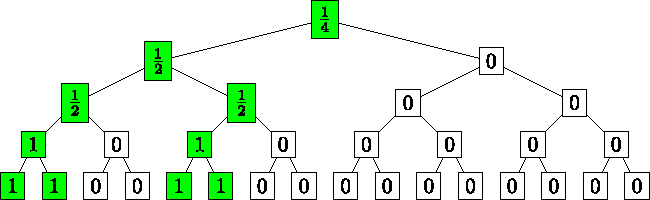
\includegraphics[width=\linewidth,height=0.78\textheight,keepaspectratio]{ccc2025-20-svg-03.pdf}\par

Figure 4.1: Subset Martingale Construction (Construction 4.5).



\emph{See Figure 4.1 for an example with $n=4$ and $B\cap[s_{0},s_{3}]=\{s_{1},s_{3}\}$. The nodes $w\in\{0,1\}^{\leq 4}$ that are colored green in the tree are those with $L(w)\subseteq B$.}\par



% END-SOURCE-ID S4.Thmtheorem5



In the following lemma, $\mathsf{UE}$ is the exponential ($2^{O(n)}$ time) version of $\mathsf{UP}$, $\mathsf{NE}$ is the exponential version of $\mathsf{NP}$, and $\mathsf{SPE}$ is the exponential version of $\mathsf{SPP}$.\par



% SOURCE-ID S4.Thmtheorem6


\par\medskip\noindent\textbf{
\textbf{Lemma 4.6}\textbf{.}
}\par



\begin{enumerate}


\item[] 
1. 


\emph{If }$B\in\mathsf{UE}$\emph{, then Construction }4.5\emph{ produces a uniform family of }${\mathsf{\#}\mathsf{P}}$\emph{-martingales.}\par





\item[] 
2. 


\emph{If }$B\in\mathsf{NE}$\emph{, then Construction }4.5\emph{ produces a uniform family of }$\mathsf{SpanP}$\emph{-martingales.}\par





\item[] 
3. 


\emph{If }$B\in\mathsf{SPE}$\emph{, then Construction }4.5\emph{ produces a uniform family of }$\mathsf{GapP}$\emph{-martingales.}\par





\end{enumerate}



% END-SOURCE-ID S4.Thmtheorem6



\par\medskip\noindent\textbf{Proof of Lemma 4.6.}\par




If $B\in\mathsf{UE}$, then we claim $A\in\mathsf{UP}$. Given $w\in\{0,1\}^{n}$, for each $i<n$, if $w[i]=1$, guess a witness for $s_{i}\in B$. If all witnesses are found, accept $w$. Because $A$ has unique witnesses, $B$ also has unique witnesses. Because the $s_{i}$’s have length logarithmic in the length of $w$, the total length of the witness for $w\in B$ is at most $|w|2^{O(\log|w|)}=|w|^{O(1)}$.
Therefore Construction 4.1 produces a uniform family of ${\mathsf{\#}\mathsf{P}}$-martingales.\par




The other two cases follow similarly.
$\blacktriangleleft$\par



% SOURCE-ID S4.Thmtheorem7


\par\medskip\noindent\textbf{
\textbf{Lemma 4.7}\textbf{.}
}\par



\emph{Let $B\subseteq\{0,1\}^{*}$ and assume the series $\sum\limits_{n=0}^{\infty}2^{c_{B}(n)-n}$ is $\mathsf{P}$-convergent.}\par


\begin{enumerate}


\item[] 
1. 


\emph{If }$B\in\mathsf{UE}$\emph{, then
the class of all infinite subsets of }$B$\emph{ has }${\mathsf{\#}\mathsf{P}}$\emph{-measure 0.}\par





\item[] 
2. 


\emph{If }$B\in\mathsf{NE}$\emph{, then
the class of all infinite subsets of }$B$\emph{ has }$\mathsf{SpanP}$\emph{-measure 0.}\par





\item[] 
3. 


\emph{If }$B\in\mathsf{SPE}$\emph{, then
the class of all infinite subsets of }$B$\emph{ has }$\mathsf{GapP}$\emph{-measure 0.}\par





\end{enumerate}



% END-SOURCE-ID S4.Thmtheorem7




\par\medskip\noindent\textbf{Proof.}\par




Combine Lemma 4.7 and the Counting Measure Borel-Cantelli Lemma (Lemma 3.13).
$\blacktriangleleft$\par



% SOURCE-ID S4.Thmtheorem8


\par\medskip\noindent\textbf{
\textbf{Corollary 4.8}\textbf{.}
}\par



\begin{enumerate}


\item[] 
1. 


\emph{Every }${\mathsf{\#}\mathsf{P}}$\emph{-random language is not in }$\mathsf{UE}$\emph{.}\par





\item[] 
2. 


\emph{Every }$\mathsf{SpanP}$\emph{-random language is not in }$\mathsf{NE}$\emph{.}\par





\item[] 
3. 


\emph{Every }$\mathsf{GapP}$\emph{-random language is not in }$\mathsf{SPE}$\emph{.}\par





\end{enumerate}



% END-SOURCE-ID S4.Thmtheorem8




\par\medskip\noindent\textbf{Proof.}\par




Let $R$ be ${\mathsf{\#}\mathsf{P}}$-random. Since $R$ is also $\mathsf{P}$-random, it satisfies the law of large numbers [51] and $c_{R}(n)\leq(\frac{1}{2}+\epsilon)n$ for all sufficiently large $n$. The previous lemma applies to contradict the ${\mathsf{\#}\mathsf{P}}$-randomness of $R$. The proofs for $\mathsf{SpanP}$-random and $\mathsf{GapP}$-random languages are analogous.
$\blacktriangleleft$\par






\par\medskip\noindent\textbf{
4.4 Acceptance Probability Construction}\par




Determining the $\mathsf{P}$-measure of $\mathsf{BPP}$ is an open problem. Van Melkebeek [77] used the weak derandomization of $\mathsf{BPP}$ from the uniform hardness assumption $\mathsf{BPP}\neq\mathsf{EXP}$ [36]
to prove a zero-one law for the $\mathsf{P}$-measure of $\mathsf{BPP}$:
either $\mu_{\mathsf{P}}(\mathsf{BPP})=0$ or $\mathsf{BPP}=\mathsf{EXP}$.
Since $\mathsf{BPP}=\mathsf{EXP}$ is equivalent to $\mu(\mathsf{BPP}\mid\mathsf{EXP})=1$ [67], it follows that determining the $\mathsf{P}$-measure of $\mathsf{BPP}$ is equivalent to resolving the $\mathsf{BPP}$ versus $\mathsf{EXP}$ problem. However, in this section we will show that $\mathsf{BPP}$ has ${\mathsf{\#}\mathsf{P}}$-measure 0. We will also show that $\mathsf{BQP}$ has $\mathsf{GapP}$-measure 0 by building on the work of Fortnow and Rogers [22, 23] that $\mathsf{BQP}\subseteq\mathsf{AWPP}$. Both of these results will be proved using the following martingale construction that tracks acceptance probabilities of classical or quantum machines.\par



% SOURCE-ID S4.Thmtheorem9


\par\medskip\noindent\textbf{
\textbf{Construction 4.9}\textbf{ }(Acceptance Probability Martingale)\textbf{.}
}\par



\emph{Let $f:\{0,1\}^{*}\times\{0,1\}\to\mathbb{N}$ be a function such that for some function $q(n)$ and all $x\in\{0,1\}^{*}$,}\par


\[\begin{gathered}
f(x,0)+f(x,1)=2^{q(|x|)}.
\end{gathered}\]


\emph{For each $w\in\{0,1\}^{*}$, let $n=|w|$ and define}\par


\[\begin{gathered}
M(w)=\prod_{i=0}^{n-1}2f(s_{i},w[i])=2^{n}\prod_{i=0}^{n-1}f(s_{i},w[i]),
\end{gathered}\]


\[\begin{gathered}
N(w)=\prod_{i=0}^{n-1}2^{q(|s_{i}|)}=2^{\sum\limits_{i=0}^{n-1}q(|s_{i}|)},
\end{gathered}\]


\emph{and}\par


\[\begin{gathered}
d(w)=\frac{M(w)}{N(w)}=2^{n}\prod_{i=0}^{n-1}\frac{f(s_{i},w[i])}{2^{q(|s_{i}|)}}.
\end{gathered}\]


\emph{Then $d$ is a martingale with $d(\lambda)=1$.}\par



\par\noindent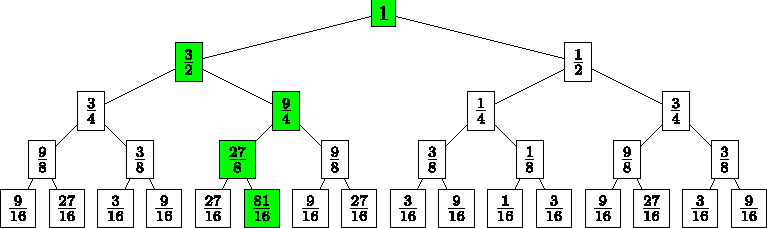
\includegraphics[width=\linewidth,height=0.78\textheight,keepaspectratio]{ccc2025-20-svg-04.pdf}\par

Figure 4.2: Acceptance Probability Martingale Construction (Construction 4.9).



\emph{See Figure 4.2 for an example with $n=4$, $A\cap[s_{0},s_{3}]=\{s_{1},s_{3}\}$, and correctness probability $\tfrac{3}{4}$. The green path highlights the prefix 0101 of the characertistic sequence of $A$.}\par



% END-SOURCE-ID S4.Thmtheorem9



For example, the function $f$ in Construction 4.9 could be the ${\mathsf{\#}\mathsf{P}}$ function where $f(x,0)$ is the number of rejecting paths and $f(x,1)$ is the number of accepting paths in a $\mathsf{PTM}$ $Q$ on input $x$. Let $q(n)$ be the random seed length of $Q$. Then\par


\[\begin{gathered}
\frac{f(x,0)}{2^{q(|x|)}}=\mathsf{Pr}[Q\textrm{ rejects }x]=\mathsf{Pr}[Q(x)=0],
\end{gathered}\]


\[\begin{gathered}
\frac{f(x,1)}{2^{q(|x|)}}=\mathsf{Pr}[Q\textrm{ accepts }x]=\mathsf{Pr}[Q(x)=1],
\end{gathered}\]


and\par


\[\begin{gathered}
d(w)=2^{n}\prod_{i=0}^{n-1}\mathsf{Pr}[Q(s_{i})=w[i]].
\end{gathered}\]


In particular, if $A\in\mathsf{BPE}=\mathsf{BPTIME}(2^{O(n)})$, then for some $c\geq 1$, there exists a $2^{cn}$-time $\mathsf{PTM}$ $Q$ that decides $A$ with error probability at most $2^{-2n}$, where the random seed length is $q(n)=2^{cn}$.\par



% SOURCE-ID S4.Thmtheorem10


\par\medskip\noindent\textbf{
\textbf{Lemma 4.10}\textbf{.}
}\par



\emph{If $A\in\mathsf{BPE}$, then the martingale $d$ produced by Construction 4.9 is a ${\mathsf{\#}\mathsf{P}}$-martingale that $0$-succeeds on $A$.}\par



% END-SOURCE-ID S4.Thmtheorem10



\par\medskip\noindent\textbf{Proof of Lemma 4.10.}\par




Let $t(n)=2^{cn}$ and $p(n)=2n$. Then
$M(w)$ is ${\mathsf{\#}\mathsf{P}}$-computable with run time on the order of\par


\[\begin{gathered}
\sum_{i=0}^{n-1}t(|s_{i}|)\leq n\cdot t(|s_{n}|)\leq n2^{c\log n}=n^{c+1}.
\end{gathered}\]


Similarly,
$N(w)$ is computable in $O(n^{c+1})$ time. Therefore $d$ is a ${\mathsf{\#}\mathsf{P}}$-martingale.
Finally, we have\par


\[\begin{gathered}
d(A\negthinspace\upharpoonright\negthinspace n)=\frac{M(A\negthinspace\upharpoonright\negthinspace n)}{N(A\negthinspace\upharpoonright\negthinspace n)}=2^{n}\prod_{i=0}^{n-1}\mathsf{Pr}[M(s_{i})=A[i]]\geq 2^{n}\prod_{i=0}^{n-1}(1-2^{-p(|s_{i}|)})
\end{gathered}\]


Using $1-x\approx e^{-x}$, we have $d(A\negthinspace\upharpoonright\negthinspace n)=\Omega(2^{n})$ because\par


\[\begin{gathered}
2^{n}\prod_{i=0}^{n-1}e^{2^{-p(|s_{i}|)}}=2^{n}e^{\sum\limits_{i=0}^{n-1}2^{-p(|s_{i}|)}}=\Omega(2^{n})
\end{gathered}\]


The last line holds because\par


\[\begin{gathered}
\sum_{i=0}^{\infty}2^{-p(|s_{i}|)}=\sum_{n=0}^{\infty}2^{n}\cdot 2^{-2n}
\end{gathered}\]


converges. Therefore $d$ $0$-succeeds on $A$.
$\blacktriangleleft$\par




Analogously, one can handle $\mathsf{BQE}=\mathsf{BQTIME}(2^{O(n)})$ [5, 16]
with $\mathsf{GapP}$ functions. For this, we need the class $\mathsf{AWPP}$ that was introduced by Fenner, Fortnow, Kurtz, and Li [19].
The following definition is due to Fenner [20]. See [18, 22, 20] for more details.\par



% SOURCE-ID S4.Thmtheorem11


\par\medskip\noindent\textbf{
\textbf{Definition 4.11}\textbf{.}
}\par



\emph{The class $\mathsf{AWPP}$ (almost-wide probabilistic polynomial-time) consists of
the languages $L$ such that for all polynomials $r$, there is a polynomial $t$ and a $\mathsf{GapP}$
function $g$ such that, for all $n$, for all $x\in\{0,1\}^{n}$,}\par


\begin{itemize}


\item[] 
$\blacksquare$ 


\emph{if }$x\in L$\emph{ then }$1-2^{-r(n)}\leq\frac{g(x)}{2^{t(n)}}\leq 1$\emph{,}\par





\item[] 
$\blacksquare$ 


\emph{if }$x\not\in L$\emph{ then }$0\leq\frac{g(x)}{2^{t(n)}}\leq 2^{-r(n)}$\emph{.}\par





\end{itemize}



% END-SOURCE-ID S4.Thmtheorem11



We define an exponential version $\mathsf{AWPE}$ by allowing $g$ to be computable in time $2^{O(n)}$ in the definition above. The class $\mathsf{GapE}$ is defined just like $\mathsf{GapP}$ but using $\mathsf{PTM}$s that run in $2^{O(n)}$ time.\par



% SOURCE-ID S4.Thmtheorem12


\par\medskip\noindent\textbf{
\textbf{Definition 4.12}\textbf{.}
}\par



\emph{The class $\mathsf{AWPE}$ (almost-wide probabilistic exponential-time) consists of
the languages $L$ such that for all $r(n)=2^{O(n)}$, there is $t(n)=2^{O(n)}$ and a $\mathsf{GapE}$
function $g$ such that, for all $n$, for all $x\in\{0,1\}^{n}$,}\par


\begin{itemize}


\item[] 
$\blacksquare$ 


\emph{if }$x\in L$\emph{ then }$1-2^{-r(n)}\leq\frac{g(x)}{2^{t(n)}}\leq 1$\emph{,}\par





\item[] 
$\blacksquare$ 


\emph{if }$x\not\in L$\emph{ then }$0\leq\frac{g(x)}{2^{t(n)}}\leq 2^{-r(n)}$\emph{.}\par





\end{itemize}



% END-SOURCE-ID S4.Thmtheorem12


% SOURCE-ID S4.Thmtheorem13


\par\medskip\noindent\textbf{
\textbf{Theorem 4.13}\textbf{.}
}\par



\emph{If $A\in\mathsf{AWPE}$, then Construction 4.9 is a $\mathsf{GapP}$-martingale that $0$-succeeds on $A$.}\par



% END-SOURCE-ID S4.Thmtheorem13




\par\medskip\noindent\textbf{Proof of Theorem 4.13.}\par




Assume $A\in\mathsf{AWPE}$, pick $r(n)=2^{n}$, and let $t(n)=2^{cn}$, and $g\in\mathsf{GapE}$ be the corresponding functions from the definition of $\mathsf{AWPE}$ such that for all $n$ and for all $x\in\{0,1\}^{n}$,\par


\begin{itemize}


\item[] 
$\blacksquare$ 


if $x\in A$, then $1-2^{-r(n)}\leq\frac{g(x)}{2^{t(n)}}\leq 1$,\par





\item[] 
$\blacksquare$ 


if $x\notin A$, then $0\leq\frac{g(x)}{2^{t(n)}}\leq 2^{-r(n)}$.\par





\end{itemize}


To adapt the acceptance probability construction, define $f(x,0)=2^{t(n)}-g(x)$ and $f(x,1)=g(x)$, and define\par


\[\begin{gathered}
M(w)=\prod_{i=0}^{n-1}2f(s_{i},w[i])=2^{n}\prod_{i=0}^{n-1}f(s_{i},w[i])
\end{gathered}\]


An argument similar to the proof of Lemma 4.10 together with the closure properties of $\mathsf{GapP}$ [18] shows that $M$ computes a $\mathsf{GapP}$ function.
Also define\par


\[\begin{gathered}
N(w)=\prod_{i=0}^{n-1}2^{t(|w_{i}|)}
\end{gathered}\]


Now we have\par


\[\begin{gathered}
d(A\negthinspace\upharpoonright\negthinspace n)=\frac{M(A\negthinspace\upharpoonright\negthinspace n)}{N(A\negthinspace\upharpoonright\negthinspace n)}=2^{n}\prod_{i=0}^{n-1}\frac{f(s_{i},w[i])}{2^{t(|w_{i}|)}}\geq 2^{n}\prod_{i=0}^{n-1}(1-2^{-r(|s_{i}|)})
\end{gathered}\]


Using $1-x\approx e^{-x}$, this yields $d(A\negthinspace\upharpoonright\negthinspace n)=\Omega(2^{n})$ because\par


\[\begin{gathered}
2^{n}\prod_{i=0}^{n-1}e^{2^{-r(|s_{i}|)}}=2^{n}e^{\sum\limits_{i=0}^{n-1}2^{-r(|s_{i}|)}}=\Omega(2^{n})
\end{gathered}\]


Therefore $d$ $0$-succeeds on $A$.
$\blacktriangleleft$
A straightforward extension of Fortnow and Rogers’ proof that $\mathsf{BQP}\subseteq\mathsf{AWPP}$ to exponential-time classes shows that
$\mathsf{BQE}\subseteq\mathsf{AWPE}$.
Combining this with Theorem 4.13 gives us the following result.\par



% SOURCE-ID S4.Thmtheorem14


\par\medskip\noindent\textbf{
\textbf{Theorem 4.14}\textbf{.}
}\par



\emph{If $A\in\mathsf{BQE}$, then there is a $\mathsf{GapP}$-martingale that $0$-succeeds on $A$.}\par



% END-SOURCE-ID S4.Thmtheorem14



Lutz [52] showed that $\mathsf{DTIME}(2^{cn})$ has $\mathsf{P}$-dimension 0 for all $c\geq 1$.
Using the above results and the Counting Measure Union lemma 3.11, we can extend this result to $\mathsf{BPTIME}$ and $\mathsf{BQTIME}$ under ${\mathsf{\#}\mathsf{P}}$ and $\mathsf{GapP}$ dimensions.\par



% SOURCE-ID S4.Thmtheorem15


\par\medskip\noindent\textbf{
\textbf{Corollary 4.15}\textbf{.}
}\par



\emph{For all $c\geq 1$,}\par


\begin{enumerate}


\item[] 
1. 


$\mathsf{BPTIME}(2^{cn})$\emph{ has }${\mathsf{\#}\mathsf{P}}$\emph{-dimension 0.}\par





\item[] 
2. 


$\mathsf{BQTIME}(2^{cn})$\emph{ has }$\mathsf{GapP}$\emph{-dimension 0.}\par





\end{enumerate}



% END-SOURCE-ID S4.Thmtheorem15


% SOURCE-ID S4.Thmtheorem16


\par\medskip\noindent\textbf{
\textbf{Corollary 4.16}\textbf{.}
}\par



\begin{enumerate}


\item[] 
1. 


$\mathsf{BPP}$\emph{ has }${\mathsf{\#}\mathsf{P}}$\emph{-dimension 0.}\par





\item[] 
2. 


$\mathsf{BQP}$\emph{ has }$\mathsf{GapP}$\emph{-dimension 0.}\par





\end{enumerate}



% END-SOURCE-ID S4.Thmtheorem16



We have the following Corollary to this section as a companion to Corollary 4.8.\par



% SOURCE-ID S4.Thmtheorem17


\par\medskip\noindent\textbf{
\textbf{Corollary 4.17}\textbf{.}
}\par



\begin{enumerate}


\item[] 
1. 


\emph{Every }${\mathsf{\#}\mathsf{P}}$\emph{-random oracle is not in }$\mathsf{BPE}$\emph{.}\par





\item[] 
2. 


\emph{Every }$\mathsf{GapP}$\emph{-random oracle is not in }$\mathsf{BQE}$\emph{.}\par





\end{enumerate}



% END-SOURCE-ID S4.Thmtheorem17





\par\medskip\noindent\textbf{
4.5 Bi-immunity Martingale Construction}\par




Mayordomo [59] showed that $\mathsf{P}$-random languages are $\mathsf{E}$-bi-immune. We extend her construction to show that $\mathsf{GapP}$-random languages are $\mathsf{SPE}$-immune, where $\mathsf{SPE}$ is the exponential analogue of $\mathsf{SPP}$.
The same construction also shows ${\mathsf{\#}\mathsf{P}}$-random languages are $\mathsf{UE}\cap\mathsf{co}\mathsf{UE}$-bi-immune and $\mathsf{SpanP}$-random languages are $\mathsf{NE}\cap\mathsf{co}\mathsf{NE}$-bi-immune.\par



% SOURCE-ID S4.Thmtheorem18


\par\medskip\noindent\textbf{
\textbf{Construction 4.18}\textbf{ }(Bi-immunity Martingale)\textbf{.}
}\par



\emph{Let $A\subseteq\{0,1\}^{*}$. Define a martingale $d$ by $d(\lambda)=1$ and for all $w\in\{0,1\}^{*}$,}\par


\[\begin{gathered}
d(w1)=\begin{cases}2d(w)&\textrm{if }s_{|w|}\in A\\
d(w)&\textrm{if }s_{|w|}\not\in A\end{cases}
\end{gathered}\]


\emph{and}\par


\[\begin{gathered}
d(w0)=\begin{cases}0&\textrm{if }s_{|w|}\in A\\
d(w)&\textrm{if }s_{|w|}\not\in A.\end{cases}
\end{gathered}\]


\emph{For all $w\in\{0,1\}^{*}$, writing $L(w)=\{s_{i}\mid w[i]=1\}$,
note we have}\par


\[\begin{gathered}
d(w)=2^{\#_{1}(A\thinspace\negthinspace\upharpoonright\negthinspace\thinspace n)}
\end{gathered}\]


\emph{if $A\subseteq L(w)$ and $d(w)=0$ otherwise.}\par



\par\noindent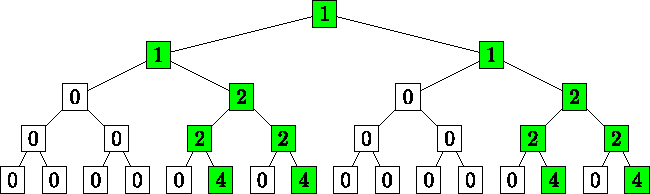
\includegraphics[width=\linewidth,height=0.78\textheight,keepaspectratio]{ccc2025-20-svg-05.pdf}\par

Figure 4.3: Bi-immunity Martingale Construction (Construction 4.18).



\emph{See Figure 4.3 for an example with $n=4$ and $A\cap[s_{0},s_{3}]=\{s_{1},s_{3}\}$. The nodes $w\in\{0,1\}^{\leq 4}$ that are colored green in the tree are those with $A\subseteq L(w)$.}\par



% END-SOURCE-ID S4.Thmtheorem18



Mayordomo [59] showed that if $A\in\mathsf{E}$, then Construction 4.18 is a $\mathsf{P}$-martingale and for any infinite language $A$, Construction 4.18 succeeds on all languages that contain $A$, as characterized by the set $S^{\infty}[d]=\{B\mid A\subseteq B\}$.\par



% SOURCE-ID S4.Thmtheorem19


\par\medskip\noindent\textbf{
\textbf{Lemma 4.19}\textbf{.}
}\par



\begin{enumerate}


\item[] 
1. 


\emph{If }$A\in\mathsf{UE}\cap\mathsf{co}\mathsf{UE}$\emph{, then Construction }4.18\emph{ is a }${\mathsf{\#}\mathsf{P}}$\emph{-martingale.}\par





\item[] 
2. 


\emph{If }$A\in\mathsf{NE}\cap\mathsf{co}\mathsf{NE}$\emph{, then Construction }4.18\emph{ is a }$\mathsf{SpanP}$\emph{-martingale.}\par





\item[] 
3. 


\emph{If }$A\in\mathsf{SPE}$\emph{, then Construction }4.18\emph{ is a }$\mathsf{GapP}$\emph{-martingale.}\par





\end{enumerate}



% END-SOURCE-ID S4.Thmtheorem19



\par\medskip\noindent\textbf{Proof of Lemma 4.19.}\par




For parts 1 and 2, on input $w$, for each $i<|w|$, guess whether $s_{i}\in A$ or $s_{i}\not\in A$ and a witness that proves this.
Note that the witnesses have total length $2^{O(n)}$ which is polynomial in $|w|$. If witnesses are found for all $s_{i}$ and prove that $A\negthinspace\upharpoonright\negthinspace|w|\subseteq L(w)$, output $d(w)=2^{|A\;\negthinspace\upharpoonright\negthinspace\;|w||}$; otherwise output $0$.\par


\begin{itemize}


\item[] 
$\blacksquare$ 


If $A\in\mathsf{UE}\cap\mathsf{co}\mathsf{UE}$, then $d$ is a $\mathsf{UPSV}$ function which can be implemented by a ${\mathsf{\#}\mathsf{P}}$ martingale.\par





\item[] 
$\blacksquare$ 


If $A\in\mathsf{NE}\cap\mathsf{co}\mathsf{NE}$, then $d$ is a $\mathsf{NPSV}$ function which can be implemented by a $\mathsf{SpanP}$ martingale.\par





\end{itemize}


For part 3, let $g\in\mathsf{GapE}$ such that $g(x)=1$ if $x\in A$ and $g(x)=0$ if $x\not\in A$. Define\par


\[\begin{gathered}
\displaystyle f(w,1) \displaystyle= \displaystyle 1+g(s_{|w|}) \\
\displaystyle f(w,0) \displaystyle= \displaystyle 1-g(s_{|w|})
\end{gathered}\]


for all $w\in\{0,1\}^{*}$. Then $f\in\mathsf{GapP}$ and\par


\[\begin{gathered}
d(wb)=2f(w,b)d(w)
\end{gathered}\]


for all $w\in\{0,1\}^{*}$ and $b\in\{0,1\}$. Therefore\par


\[\begin{gathered}
d(w)=2^{|w|}\prod_{i=0}^{|w|-1}f(w\negthinspace\upharpoonright\negthinspace i,w[i])
\end{gathered}\]


is a $\mathsf{GapP}$ function.
$\blacktriangleleft$\par



% SOURCE-ID S4.Thmtheorem20


\par\medskip\noindent\textbf{
\textbf{Corollary 4.20}\textbf{.}
}\par



\begin{enumerate}


\item[] 
1. 


\emph{Every }${\mathsf{\#}\mathsf{P}}$\emph{-random language is }$\mathsf{UE}\cap\mathsf{co}\mathsf{UE}$\emph{-bi-immune.}\par





\item[] 
2. 


\emph{Every }$\mathsf{SpanP}$\emph{-random language is }$\mathsf{NE}\cap\mathsf{co}\mathsf{NE}$\emph{-bi-immune.}\par





\item[] 
3. 


\emph{Every }$\mathsf{GapP}$\emph{-random language is }$\mathsf{SPE}$\emph{-bi-immune.}\par





\end{enumerate}



% END-SOURCE-ID S4.Thmtheorem20




\par\medskip\noindent\textbf{Proof of Corollary 4.20.}\par




Let $R$ be $\mathsf{GapP}$-random and let $A\in\mathsf{SPE}$. By the previous two lemmas, $R$ is $A$-immune. Since $\mathsf{SPE}$ is closed under complement, $R^{c}$ is also $A$-immune. The other two parts are analogous.
$\blacktriangleleft$
Since $\mathsf{SPP}$ contains the counting classes $\mathsf{UP}$, $\mathsf{FewP}$, and $\mathsf{Few}$, $\mathsf{GapP}$-random languages are also immune to these classes.\par







\par\medskip\noindent\textbf{
5 Entropy Rates and Kolmogorov Complexity}\par




We will use the Cover Martingale and Conditional Expectation Martingale Constructions (Constructions 4.1 and 4.3) to develop a few tools for working with counting measures and dimensions. First, we extend the entropy rates used by Hitchcock and Vinodchandran [35] to our setting. Then we extend Lutz’s results on Kolmogorov complexity and $\mathsf{PSPACE}$-measure to counting measure.\par




\par\medskip\noindent\textbf{
5.1 Entropy Rates}\par




We will show in this section that the Cover Martingale Construction (Construction 4.1) may be combined with the concept of entropy rates to build counting martingales.\par



% SOURCE-ID S5.Thmtheorem1


\par\medskip\noindent\textbf{
\textbf{Definition 5.1}\textbf{.}
}\par



\emph{The entropy
rate of a language $A\subseteq\{0,1\}^{*}$
is}\par


\[\begin{gathered}
H_{A}=\limsup\limits_{n\to\infty}\frac{\log|A_{=n}|}{n}.
\end{gathered}\]



% END-SOURCE-ID S5.Thmtheorem1



Intuitively, $H_{A}$ gives an asymptotic measurement of the amount by
which every string in $A_{=n}$ is compressed in an optimal code [43].
The \emph{i.o.-class
of $A$} is\par


\[\begin{gathered}
A^{\mathsf{i.o.}}=\{S\in\mathsf{C}\mid(\exists^{\infty}n)\ S\negthinspace\upharpoonright\negthinspace n\in A\}.
\end{gathered}\]


That is, $A^{\mathsf{i.o.}}$ is the class of sequences that have infinitely many
prefixes in $A$.\par



% SOURCE-ID S5.Thmtheorem2


\par\medskip\noindent\textbf{
\textbf{Definition 5.2}\textbf{ }(Hitchcock and Vinodchandran [35])\textbf{.}
}\par



\emph{Let ${\cal C}$ be a class of languages and $X\subseteq\mathsf{C}$. The ${\cal C}$-entropy rate of $X$ is}\par


\[\begin{gathered}
{\cal H}_{\cal C}(X)=\inf\{H_{A}\mid A\in{\cal C}\textrm{ and }X\subseteq A^{\mathsf{i.o.}}\}.
\end{gathered}\]



% END-SOURCE-ID S5.Thmtheorem2



Informally, ${\cal H}_{\cal C}(X)$ is the lowest entropy rate with which every
element of $X$ can be covered infinitely often by a language in
${\cal C}$.
We may also interpret ${\cal H}_{\cal C}(X)$ as a notion of dimension.
For all $X\subseteq\mathsf{C}$, it is known that
${\mathsf{dim}}_{\mathsf{H}}(X)={\cal H}_{\mathsf{ALL}}(X),$ where $\mathsf{ALL}$ is the class of all
languages and ${\mathsf{dim}}_{\mathsf{H}}$ is Hausdorff dimension (see [68, 72]). Hitchcock [30, 28] showed that using other
classes gives equivalent definitions of the constructive dimension ($\mathsf{cdim}(X)={\cal H}_{\mathsf{CE}}(X)$), computable dimension (${\mathsf{dim}}_{\mathsf{comp}}(X)={\cal H}_{\mathsf{DEC}}(X)$), and polynomial-space dimension (${\mathsf{dim}}_{\mathsf{PSPACE}}(X)={\cal H}_{\mathsf{PSPACE}}(X)$).
For time-bounded dimension, no analogous result is known.
However, the following upper bound is true [30, 28]:
for all $X\subseteq\mathsf{C}$, ${\cal H}_{\mathsf{P}}(X)\leq{\mathsf{dim}}_{\mathsf{P}}(X).$\par




The $\mathsf{NP}$-entropy rate is an upper bound for
${\Delta^{\mathsf{P}}_{3}}$-dimension.\par



% SOURCE-ID S5.Thmtheorem3


\par\medskip\noindent\textbf{
\textbf{Theorem 5.3}\textbf{ }(Hitchcock and Vinodchandran [35])\textbf{.}
}\par



\emph{For all $X\subseteq\mathsf{C}$,}\par


\[\begin{gathered}
{\mathsf{dim}}_{\Delta^{\mathsf{P}}_{3}}(X)\leq{\cal H}_{\mathsf{NP}}(X).
\end{gathered}\]



% END-SOURCE-ID S5.Thmtheorem3



We now show that the $\mathsf{NP}$-entropy rate upper bounds $\mathsf{SpanP}$-dimension. Analogously, the $\mathsf{UP}$-entropy rate upper bounds ${\mathsf{\#}\mathsf{P}}$-dimension and the $\mathsf{SPP}$-entropy rate upper bounds $\mathsf{GapP}$-dimension. The proof uses Construction 4.1 and Lemma 4.2.\par



% SOURCE-ID S5.Thmtheorem4


\par\medskip\noindent\textbf{
\textbf{Theorem 5.4}\textbf{.}
}\par



\emph{For all $X\subseteq\mathsf{C}$,}\par


\begin{enumerate}


\item[] 
1. 


${\mathsf{dim}}_{\mathsf{\#}\mathsf{P}}(X)\leq{\cal H}_{\mathsf{UP}}(X)\leq{\cal H}_{\mathsf{P}}(X)$\emph{}\par





\item[] 
2. 


${\mathsf{dim}}_{\mathsf{SpanP}}(X)\leq{\cal H}_{\mathsf{NP}}(X).$\emph{}\par





\item[] 
3. 


${\mathsf{dim}}_{\mathsf{GapP}}(X)\leq{\cal H}_{\mathsf{SPP}}(X).$\emph{}\par





\end{enumerate}



% END-SOURCE-ID S5.Thmtheorem4



\par\medskip\noindent\textbf{Proof of Theorem 5.4.}\par




We prove the second inequality, the proofs of the other inequalities are analogous.\par




Let $\alpha>{\cal H}_{\mathsf{NP}}(X)$ and $\epsilon>0$ such that $2^{\alpha}$ and
$2^{\epsilon}$ are rational. Let $A\in\mathsf{NP}$ such that $X\subseteq A^{\mathsf{i.o.}}$ and $H_{A}<\alpha$. We can assume that $|A_{=n}|\leq 2^{\alpha n}$ for all $n$. It suffices to show that ${\mathsf{dim}}_{\mathsf{SpanP}}(X)\leq\alpha+\epsilon$.\par




We use Construction 4.1 and Lemma 4.2 to obtain a uniform family $(d_{n}\mid n\geq 0)$ of $\mathsf{SpanP}$ martingales with\par


\[\begin{gathered}
d_{n}(\lambda)=\frac{|A_{=n}|}{2^{n}}\leq 2^{(\alpha-1)n}
\end{gathered}\]


and $d_{n}(v)=1$ for all $v\in A_{=n}$. We now apply the Counting Dimension Borel-Cantelli Lemma (Lemma 3.14) to complete the proof.
$\blacktriangleleft$\par




We note that combining Theorems 5.4 and 3.17 gives a new proof of Theorem 5.3.\par




We will next extend Theorem 5.4 to the measure setting. First, we define an entropy rate version of measure 0. The idea in this definition is to extend the entropy rate ${\cal H}_{\cal C}$ to define a measure ${{\cal M}_{{\cal C}}}$.\par



% SOURCE-ID S5.Thmtheorem5


\par\medskip\noindent\textbf{
\textbf{Definition 5.5}\textbf{ }(Entropy Rate Measure)\textbf{.}
}\par



\emph{Let $X\subseteq\mathsf{C}$ and let ${\cal C}$ be a complexity class.
If there exist $A\in{\cal C}$ and $f\in\mathsf{FP}$ such that}\par


\begin{enumerate}


\item[] 
1. 


$X\subseteq A^{\mathsf{i.o.}}$\emph{,}\par





\item[] 
2. 


$\log|A_{=n}|<n-f(n)$\emph{ for sufficiently large }$n$\emph{, and}\par





\item[] 
3. 


$\sum\limits_{n=0}^{\infty}2^{-f(n)}$\emph{ is }$\mathsf{P}$\emph{-convergent,}\par





\end{enumerate}


\emph{then $X$ has ${{\cal M}_{{\cal C}}}$-measure 0 and we write ${{\cal M}_{{\cal C}}}(X)=0$.}\par



% END-SOURCE-ID S5.Thmtheorem5



We observe that ${{\cal M}_{{\cal C}}}$-measure has many of the standard measure properties. When using ${\cal C}=\mathsf{ALL}$, the class of all languages, it refines Lebesgue measure: if ${{\cal M}_{\mathsf{ALL}}}(X)=0$, then $X$ has Lebesgue measure 0. Using ${\cal C}=\mathsf{PSPACE}$, we have if ${{\cal M}_{\mathsf{PSPACE}}}(X)=0$, then $\mu_{\mathsf{PSPACE}}(X)=0$.\par



% SOURCE-ID S5.Thmtheorem6


\par\medskip\noindent\textbf{
\textbf{Proposition 5.6}\textbf{.}
}\par



\emph{Let ${\cal C},{\cal D}$ be classes of languages and
$X,Y\subseteq\mathsf{C}$.}\par


\begin{enumerate}


\item[] 
1. 


\emph{If }${\cal C}\subseteq{\cal D}$\emph{, }${{\cal M}_{{\cal C}}}(X)=0$\emph{ implies }${{\cal M}_{{\cal D}}}(X)=0$\emph{.}\par





\item[] 
2. 


\emph{If }$X\subseteq Y$\emph{, then }${{\cal M}_{{\cal C}}}(Y)=0$\emph{ implies }${{\cal M}_{{\cal C}}}(X)=0$\emph{.}\par





\item[] 
3. 


\emph{If }${\cal C}$\emph{ is closed under union, then }${{\cal M}_{{\cal C}}}(X)=0$\emph{ and }${{\cal M}_{{\cal C}}}(Y)=0$\emph{ implies }${{\cal M}_{{\cal C}}}(X\cup Y)=0$\emph{.}\par





\end{enumerate}



% END-SOURCE-ID S5.Thmtheorem6



We now establish our measure-theoretic extension of Theorem 5.4. This proof also uses Construction 4.1 and Lemma 4.2.\par



% SOURCE-ID S5.Thmtheorem7


\par\medskip\noindent\textbf{
\textbf{Theorem 5.7}\textbf{.}
}\par



\emph{Let $X\subseteq\mathsf{C}$.}\par


\begin{enumerate}


\item[] 
1. 


\emph{If }${{\cal M}_{\mathsf{UP}}}(X)=0$\emph{, then }$\mu_{\mathsf{\#}\mathsf{P}}(X)=0$\emph{.}\par





\item[] 
2. 


\emph{If }${{\cal M}_{\mathsf{NP}}}(X)=0$\emph{, then }$\mu_{\mathsf{SpanP}}(X)=0$\emph{.}\par





\item[] 
3. 


\emph{If }${{\cal M}_{\mathsf{SPP}}}(X)=0$\emph{, then }$\mu_{\mathsf{GapP}}(X)=0$\emph{.}\par





\end{enumerate}



% END-SOURCE-ID S5.Thmtheorem7




\par\medskip\noindent\textbf{Proof of Theorem 5.7.}\par




Assume ${{\cal M}_{\mathsf{NP}}}(X)=0$ and obtain the cover $A\in\mathsf{NP}$ and the function $f\in\mathsf{FP}$ satisfying the definition of ${{\cal M}_{\mathsf{NP}}}(X)=0$.
We use Construction 4.1 and Lemma 4.2 to obtain a uniform family of exact $\mathsf{SpanP}$ martingales $(d_{n}\mid n\geq 0)$ with\par


\[\begin{gathered}
d_{n}(\lambda)=\frac{|A_{=n}|}{2^{n}}\leq\frac{2^{n-f(n)}}{2^{n}}=2^{-f(n)}
\end{gathered}\]


and
$d_{n}(w)=1$ for all $w\in A_{=n}$.
The Counting Measure Borel-Cantelli lemma (Lemma 3.13) completes the proof. The proofs of the other items are analogous.
$\blacktriangleleft$\par






\par\medskip\noindent\textbf{
5.2 Kolmogorov Complexity}\par




Lutz [50] showed that the space-bounded Kolmogorov complexity class\par


\[\begin{gathered}
\{S\mid(\exists^{\infty}n)\,KS^{p}(S\negthinspace\upharpoonright\negthinspace n)<n-f(n)\}
\end{gathered}\]


has $\mathsf{PSPACE}$-measure 0 where $p$ is a polynomial, and $\sum\limits_{n=0}^{\infty}2^{-f(n)}$ is $\mathsf{P}$-convergent. In other words, if $S$ is $\mathsf{PSPACE}$-random, then $KS^{p}(S\negthinspace\upharpoonright\negthinspace n)\geq n-f(n)$ a.e. For $\mathsf{P}$-random sequences, Lutz proved that the time-bounded Kolmogorov complexity $K^{p}(S\negthinspace\upharpoonright\negthinspace n)\geq c\log n$ a.e. for any polynomial $p$.\par




We use the Conditional Expectation Martingale Construction (Construction 4.3) to obtain an intermediate result for time-bounded Kolmogorov complexity and ${\mathsf{\#}\mathsf{P}}$-measure.\par




% SOURCE-ID S5.Thmtheorem8


\par\medskip\noindent\textbf{
\textbf{Theorem 5.8}\textbf{.}
}\par



\emph{Suppose $f\in\mathsf{FP}$ and the series $\sum\limits_{n=0}^{\infty}2^{-f(n)}$ is $\mathsf{P}$-convergent.
Let $p$ be a polynomial and}\par


\[\begin{gathered}
X=\{S\mid(\exists^{\infty}n)\,K^{p}(S\negthinspace\upharpoonright\negthinspace
n)<n-f(n)\}.
\end{gathered}\]


\emph{Then $X$ has ${\mathsf{\#}\mathsf{P}}$-measure 0.}\par



% END-SOURCE-ID S5.Thmtheorem8




\par\medskip\noindent\textbf{Proof of Theorem 5.8.}\par




For each $n$, let\par


\[\begin{gathered}
X_{n}=\{x\in\{0,1\}^{n}\mid K^{p}(x)<n-f(n)\}.
\end{gathered}\]


For $w\in\{0,1\}^{\leq n}$, let\par


\[\begin{gathered}
d_{n}(w)=\mathsf{Pr}(X_{n}\mid w)=\frac{|\{x\in X_{n}\mid w\sqsubseteq x\}|}{2^{n-|w|}}.
\end{gathered}\]


This martingale satisfies\par


\[\begin{gathered}
d_{n}(\lambda)\leq\frac{|X_{n}|}{2^{n}}\leq\frac{2^{n-f(n)}}{2^{n}}=2^{-f(n)}
\end{gathered}\]


and $d_{n}(x)=1$ for all $x\in X_{n}$. However, $d_{n}$ does not appear to be a ${\mathsf{\#}\mathsf{P}}$ martingale because its numerator is a $\mathsf{SpanP}$ function.
We will upper bound the $\mathsf{SpanP}$-martingale $d_{n}$ by another martingale $d_{n}^{\prime}$ that is ${\mathsf{\#}\mathsf{P}}$-computable and still satisfies $d_{n}^{\prime}(\lambda)\leq 2^{-f(n)}.$\par




Let $U$ be a universal Turing machine and define\par


\[\begin{gathered}
C=\left\{\langle 0^{n},w,x,\pi\rangle\left|\begin{array}[]{l}w\in\{0,1\}^{\leq
n},x\in\{0,1\}^{n},\pi\in\{0,1\}^{<n-f(n)},\\
w\sqsubseteq x,\textrm{ and }U(\pi)=x\textrm{ in }\leq p(n)\textrm{ time}\end{array}\right.\right\}.
\end{gathered}\]


Then $C\in\mathsf{P}$, so the function\par


\[\begin{gathered}
g(0^{n},w)=\left|\left\{\langle x,\pi\rangle\left|\begin{array}[]{l}x\in\{0,1\}^{n},\pi\in\{0,1\}^{<n-f(n)},w\sqsubseteq x\\
\textrm{and }U(\pi)=x\textrm{ in }\leq p(n)\textrm{ time}\end{array}\right.\right\}\right|.
\end{gathered}\]


is in ${\mathsf{\#}\mathsf{P}}$.
We use Construction 4.3.
Define the ${\mathsf{\#}\mathsf{P}}$-martingale\par


\[\begin{gathered}
d_{n}^{\prime}(w)=\frac{g(0^{n},w)}{2^{n-|w|}}
\end{gathered}\]


for all $w\in\{0,1\}^{\leq n}$ and $d_{n}^{\prime}(y)=d_{n}^{\prime}(y\negthinspace\upharpoonright\negthinspace n)$ for $y\in\{0,1\}^{>n}.$
Notice that $g(0^{n},w)\leq 2^{n-f(n)}$, so $d_{n}^{\prime}(\lambda)\leq 2^{-f(n)}$.
Also, $d_{n}^{\prime}(x)\geq d_{n}(x)$ for all $x\in\{0,1\}^{*}$.
If $x\in X_{n}$, then\par


\[\begin{gathered}
g(0^{n},x)=\left|\left\{\pi\left|\begin{array}[]{l}x\in\{0,1\}^{n},\pi\in\{0,1\}^{<n-f(n)},\\
\textrm{and }U(\pi)=x\textrm{ in }\leq p(n)\textrm{ time}\end{array}\right.\right\}\right|\geq 1.
\end{gathered}\]


and $d_{n}^{\prime}(x)\geq 1=d_{n}(x).$
Therefore
$X_{n}\subseteq S^{1}[d_{n}^{\prime}].$ Also, $(d_{n}^{\prime}\mid n\in\mathbb{N})$ is exactly and uniformly ${\mathsf{\#}\mathsf{P}}$-computable by Lemma 4.4.
We apply the Counting Measure
Borel-Cantelli Lemma (Lemma 3.13)
to conclude that\par


\[\begin{gathered}
X\subseteq\bigcap_{i=0}^{\infty}\bigcup_{j\geq i}^{\infty}S^{1}[d_{n}^{\prime}]
\end{gathered}\]


has ${\mathsf{\#}\mathsf{P}}$-measure 0.
$\blacktriangleleft$\par



% SOURCE-ID S5.Thmtheorem9


\par\medskip\noindent\textbf{
\textbf{Corollary 5.9}\textbf{.}
}\par



\emph{Suppose $f\in\mathsf{FP}$ and the series $\sum\limits_{n=0}^{\infty}2^{-f(n)}$ is $\mathsf{P}$-convergent.
If $S$ is ${\mathsf{\#}\mathsf{P}}$-random, then $K^{p}(S\negthinspace\upharpoonright\negthinspace n)\geq n-f(n)$ a.e.}\par



% END-SOURCE-ID S5.Thmtheorem9



The following Theorem is a variation of Theorem 5.8 which will be used in Section 6.\par



% SOURCE-ID S5.Thmtheorem10


\par\medskip\noindent\textbf{
\textbf{Theorem 5.10}\textbf{.}
}\par



\emph{Suppose $f\in\mathsf{FP}$ and the series $\sum\limits_{n=0}^{\infty}2^{-f(n)}$ is $\mathsf{P}$-convergent.
Let $p$ be a polynomial and}\par


\[\begin{gathered}
X=\{A\mid(\exists^{\infty}n)\,K^{p}(A_{=n})<2^{n}-f(2^{n})\}.
\end{gathered}\]


\emph{Then $X$ has ${\mathsf{\#}\mathsf{P}}$-measure 0.}\par



% END-SOURCE-ID S5.Thmtheorem10




\par\medskip\noindent\textbf{Proof of Theorem 5.10.}\par




If $K^{p}(A_{=n})<2^{n}-f(2^{n})$ then we have\par


\[\begin{gathered}
\displaystyle K^{p}(A_{\leq n}) \displaystyle\leq \displaystyle K^{p}(A_{<n})+K^{p}(A_{=n})+O(n) \\
\displaystyle\leq \displaystyle 2^{n}+2^{n}-f(2^{n})+O(n) \\
\displaystyle= \displaystyle 2^{n+1}-f(2^{n})+O(n)
\end{gathered}\]


It follows from Theorem 5.8 that $X$ has ${\mathsf{\#}\mathsf{P}}$-measure 0.
$\blacktriangleleft$\par




For any $t,s:\mathbb{N}\to\mathbb{N}$, define the class\par


\[\begin{gathered}
{\cal K}^{t}(s(n))=\{S\in\mathsf{C}\mid(\exists^{\infty}n)K^{t}(S\negthinspace\upharpoonright\negthinspace n)\leq s(n)\}.
\end{gathered}\]



% SOURCE-ID S5.Thmtheorem11


\par\medskip\noindent\textbf{
\textbf{Theorem 5.11}\textbf{.}
}\par



\emph{For all $s\in[0,1]$ and polynomials $p$, ${\cal K}^{p}(sn)$ has ${\mathsf{\#}\mathsf{P}}$-dimension $s$.}\par



% END-SOURCE-ID S5.Thmtheorem11




\par\medskip\noindent\textbf{Proof of Theorem 5.11.}\par




For each $n$, let\par


\[\begin{gathered}
X_{n}=\{x\in\{0,1\}^{n}\mid K^{p}(x)\leq s|x|\}.
\end{gathered}\]


Then use Construction 4.3 as in the proof of Theorem 5.8 to obtain a ${\mathsf{\#}\mathsf{P}}$-martingale $d_{n}$ for each $n$ where $d_{n}(x)\geq 2^{(1-s)n}$ for all $x\in X_{n}.$ We then apply the Counting Dimension Borel-Cantelli Lemma (Lemma 3.14).
This shows ${\mathsf{dim}}_{{\mathsf{\#}\mathsf{P}}}({\cal K}^{P}(sn))\leq s$. The lower bound that the dimension is at least $s$ follows from previous work on Kolmogorov complexity and dimension [53, 61].
$\blacktriangleleft$\par







\par\medskip\noindent\textbf{
6 Applications}\par




This section contains our main applications. We start with classical circuit complexity, then move on to quantum circuit complexity, and lastly the density of hard sets.\par




\par\medskip\noindent\textbf{
6.1 Classical Circuit Complexity}\par




Lutz [50] showed that for all $\alpha<1$, the class\par


\[\begin{gathered}
X_{\alpha}=\mathsf{SIZE}^{\mathsf{i.o.}}\!\!\left(\frac{2^{n}}{n}\left(1+\frac{\alpha\log n}{n}\right)\right)
\end{gathered}\]


has $\mathsf{PSPACE}$-measure 0. Additionally, Lutz showed that for any $c\geq 1$ and $k\geq 1$, the classes $\mathsf{P}/cn$ and $\mathsf{SIZE}\!(n^{k})$ have polynomial-time measure 0 and quasipolynomial-time measure 0, respectively.
Mayordomo [60] used Stockmeyer’s approximate counting
of ${\mathsf{\#}\mathsf{P}}$ functions [73] to show that $\mathsf{P}/\mathsf{poly}$ has
measure 0 in the third level of the exponential hierarchy.\par




We begin by extending Lutz’s result to ${{\cal M}_{\mathsf{NP}}}$-measure, in order to improve the theorem to $\mathsf{SpanP}$-measure. The proof uses the Minimum Circuit Size Problem ($\mathsf{MCSP}$) [39] to form a cover. In $\mathsf{MCSP}$, we are given the full $2^{n}$-length truth-table of a Boolean function $f:\{0,1\}^{n}\to\{0,1\}$ and a number $s\geq 1$ and asked to decide whether there is a circuit of size at most $s$ computing $f$. The $\mathsf{MCSP}$ problem is in $\mathsf{NP}$ and not known to be $\mathsf{NP}$-complete [39, 65, 34].
The $\mathsf{MCSP}$ problem fits perfectly into the ${{\cal M}_{\mathsf{NP}}}$ framework to help improve Lutz’s result.\par



% SOURCE-ID S6.Thmtheorem1


\par\medskip\noindent\textbf{
\textbf{Theorem 6.1}\textbf{.}
}\par



\emph{For all $\alpha<1$,}\par


\[\begin{gathered}
\mathsf{SIZE}^{\mathsf{i.o.}}\!\!\left(\frac{2^{n}}{n}\left(1+\frac{\alpha\log
n}{n}\right)\right)
\end{gathered}\]


\emph{has ${{\cal M}_{\mathsf{NP}}}$-measure 0.}\par



% END-SOURCE-ID S6.Thmtheorem1



\par\medskip\noindent\textbf{Proof of Theorem 6.1.}\par




Let $s(n)=\frac{2^{n}}{n}\left(1+\frac{\alpha\log n}{n}\right)$ where $\alpha<1$ and let $X=\mathsf{SIZE}^{\mathsf{i.o.}}\!\!(s(n))$.\par




Define\par


\[\begin{gathered}
\displaystyle A \displaystyle= \displaystyle\left\{B_{\leq n}\left|\langle B_{=n},s(n)\rangle\in\mathsf{MCSP}\right.\right\} \\
\displaystyle= \displaystyle\left\{B_{\leq n}\left|B_{=n}\text{ has a circuit of size at most }s(n)\right.\right\}.
\end{gathered}\]


Then $A\in\mathsf{NP}$, $X\subseteq A^{\mathsf{i.o.}}$, and we need to show that $\log|A_{=N}|<N-f(N)$, where $N=2^{n+1}-1$, for some $f\in\mathsf{FP}$ such that $\sum_{n=0}^{\infty}2^{-f(n)}$ is $\mathsf{P}$-convergent. Using the bound in [50], we will have:\par


\[\begin{gathered}
\displaystyle\log|A_{=N}| \displaystyle< \displaystyle\sum\limits_{m=0}^{n-1}2^{m}+\log\left(48es\left(n\right)\right)^{s(n)} \\
\displaystyle= \displaystyle 2^{n}-1+s(n)\left(\log(48e)+\log\left(s\left(n\right)\right)\right) \\
\displaystyle= \displaystyle 2^{n}-1+\frac{2^{n}}{n}\left(1+\frac{\alpha\log n}{n}\right)\left(\log\left(48e\right)+n-\log n+\log\left(1+\frac{\alpha\log n}{n}\right)\right) \\
\displaystyle< \displaystyle 2^{n}-1+\frac{2^{n}}{n}\left(n+\alpha\log n-\log n+6\right) \\
\displaystyle< \displaystyle 2^{n+1}-1-\frac{2^{n}}{n}\left(1-\frac{\alpha}{2}\right)\log n \\
\displaystyle= \displaystyle N-\frac{2^{n}}{n}\left(1-\frac{\alpha}{2}\right)\log n.
\end{gathered}\]


As a result,\par


\[\begin{gathered}
\displaystyle f(N) \displaystyle= \displaystyle\left(1-\frac{\alpha}{2}\right)\frac{2^{n}}{n}\log n \\
\displaystyle= \displaystyle\left(1-\frac{\alpha}{2}\right)\frac{N+1}{2(\log\left(N+1\right)-1)}\log\left(\log\left(N+1\right)-1\right).
\end{gathered}\]


It is easy to see that $f\in\mathsf{FP}$ and $\sum_{n=0}^{\infty}2^{-f(n)}$ is $\mathsf{P}$-convergent.
$\blacktriangleleft$\par



% SOURCE-ID S6.Thmtheorem2


\par\medskip\noindent\textbf{
\textbf{Corollary 6.2}\textbf{.}
}\par



\emph{For all $\alpha<1$,
$\mathsf{SIZE}^{\mathsf{i.o.}}\!\!\left(\frac{2^{n}}{n}\left(1+\frac{\alpha\log
n}{n}\right)\right)$
has $\mathsf{SpanP}$-measure 0.}\par



% END-SOURCE-ID S6.Thmtheorem2




\par\medskip\noindent\textbf{Proof.}\par




This is immediate from Theorem 6.1 and Theorem 5.7.
$\blacktriangleleft$\par



% SOURCE-ID S6.Thmtheorem3


\par\medskip\noindent\textbf{
\textbf{Corollary 6.3}\textbf{.}
}\par



\emph{For all $\alpha<1$,
$\mathsf{SIZE}^{\mathsf{i.o.}}\!\!\left(\frac{2^{n}}{n}\left(1+\frac{\alpha\log
n}{n}\right)\right)$
has ${\Delta^{\mathsf{P}}_{3}}$-measure 0 and measure 0 in $\Delta^{\mathsf{E}}_{3}$.}\par



% END-SOURCE-ID S6.Thmtheorem3




\par\medskip\noindent\textbf{Proof.}\par




This is immediate from Corollary 6.2 and Theorem 3.17.
$\blacktriangleleft$\par




Under a derandomization hypothesis, Corollary 6.3 improves by one level in the exponential hierarchy to $\Delta^{\mathsf{E}}_{2}=\mathsf{E}^{\mathsf{NP}}$. This yields a stronger lower bound than other conditional approaches for obtaining lower bounds in $\mathsf{E}^{\mathsf{NP}}$ [1, 8].\par



% SOURCE-ID S6.Thmtheorem4


\par\medskip\noindent\textbf{
\textbf{Corollary 6.4}\textbf{.}
}\par



\emph{If Derandomization Hypothesis 2.7 is true, then
$\mathsf{SIZE}^{\mathsf{i.o.}}\!\!\left(\frac{2^{n}}{n}\left(1+\frac{\alpha\log
n}{n}\right)\right)$
has ${\Delta^{\mathsf{P}}_{2}}$-measure 0 and measure 0 in $\Delta^{\mathsf{E}}_{2}$.}\par



% END-SOURCE-ID S6.Thmtheorem4




\par\medskip\noindent\textbf{Proof.}\par




This is immediate from Corollary 6.2 and Theorem 3.19.
$\blacktriangleleft$\par




Lutz [52] showed that
for all $\alpha\in[0,1]$, the class\par


\[\begin{gathered}
{\cal D}_{\alpha}=\mathsf{SIZE}\!\left(\alpha\frac{2^{n}}{n}\right)
\end{gathered}\]


has $\mathsf{PSPACE}$-dimension $\alpha$. Hitchcock and Vinodchandran [35] showed that
${\cal H}_{\mathsf{NP}}({\cal D}_{\alpha})=\alpha,$
yielding the improvement that ${\cal D}_{\alpha}$ has ${\Delta^{\mathsf{P}}_{3}}$-dimension $\alpha$.
It is immediate from these and Theorem 5.4 that ${\cal D}_{\alpha}$ has $\mathsf{SpanP}$-dimension $\alpha$.
We can improve this to ${\mathsf{\#}\mathsf{P}}$-dimension by using a Kolmogorov complexity argument.\par



% SOURCE-ID S6.Thmtheorem5


\par\medskip\noindent\textbf{
\textbf{Theorem 6.5}\textbf{.}
}\par



\emph{For all $\alpha<1$,
${\mathsf{dim}}_{{\mathsf{\#}\mathsf{P}}}\left(\mathsf{SIZE}\!\left(\alpha\frac{2^{n}}{n}\right)\right)=\alpha.$}\par



% END-SOURCE-ID S6.Thmtheorem5




\par\medskip\noindent\textbf{Proof of Theorem 6.5.}\par




Let $X_{\alpha}=\left(\mathsf{SIZE}\!\left(\alpha\frac{2^{n}}{n}\right)\right)$ and let $B\in X_{\alpha}$.
For all sufficiently large $n$, $\langle B_{=n},s\rangle\in\mathsf{MCSP}$ for $s=\alpha\frac{2^{n}}{n}$. Let $C$ be a circuit of size $s$ on $n$ inputs. Frandsen and Miltersen [24] showed that there exists a stack program of size at most $(s+1)(c+\log(n+s))$ that constructs $C$. Let $\gamma>\beta>\alpha$ be arbitrarily close rationals. Let $p(n)=n^{3}$ and $q(n)=n^{4}$.
For all $n$ larger than some $n_{0}$,\par


\[\begin{gathered}
\displaystyle K^{p(2^{n})}(B_{=n}) \displaystyle\leq \displaystyle(s+1)(c+\log(n+s))+O(\log n) \\
\displaystyle\leq \displaystyle\left(\alpha\frac{2^{n}}{n}+1\right)\left(c+\log\left(\alpha\frac{2^{n}}{n}+n\right)\right)+O(\log n) \\
\displaystyle\leq \displaystyle\left(\beta\frac{2^{n}}{n}\right)\left(c+\log\left(\beta\frac{2^{n}}{n}\right)\right) \\
\displaystyle\leq \displaystyle\left(\beta\frac{2^{n}}{n}\right)\left(c+\log\beta+n-\log n\right) \\
\displaystyle\leq \displaystyle\left(\beta\frac{2^{n}}{n}\right)n \\
\displaystyle\leq \displaystyle\beta 2^{n}.
\end{gathered}\]


Let $N=2^{n+1}-1$. We have\par


\[\begin{gathered}
\displaystyle K^{q(N)}(B_{\leq n}) \displaystyle\leq \displaystyle\sum_{k=n_{0}}^{n}K^{p(2^{k})}(B_{=k})+O(n) \\
\displaystyle\leq \displaystyle\beta N+O(n) \\
\displaystyle\leq \displaystyle\gamma N,
\end{gathered}\]


so\par


\[\begin{gathered}
\frac{K^{q(N)}(B\negthinspace\upharpoonright\negthinspace N)}{N}\leq\gamma
\end{gathered}\]


for all sufficiently large $N$ of the form $2^{n+1}-1$. Therefore $X_{\alpha}\subseteq{\cal K}^{q}(\gamma n)$ and
${\mathsf{dim}}_{\mathsf{\#}\mathsf{P}}(X_{\alpha})\leq{\mathsf{dim}}_{\mathsf{\#}\mathsf{P}}({\cal K}^{q}(\gamma n))=\gamma$ by Theorem 5.11.
The dimension lower bound holds because ${\mathsf{dim}}_{\mathsf{\#}\mathsf{P}}(X_{\alpha})\allowbreak\geq{\mathsf{dim}}_{\mathsf{H}}(X_{\alpha})=\alpha$ [52]. The theorem follows because $\alpha$ and $\gamma$ are arbitrarily close.
$\blacktriangleleft$\par



% SOURCE-ID S6.Thmtheorem6


\par\medskip\noindent\textbf{
\textbf{Corollary 6.6}\textbf{.}
}\par



${\mathsf{P}/\mathsf{poly}}$\emph{ has ${\mathsf{\#}\mathsf{P}}$-dimension 0.}\par



% END-SOURCE-ID S6.Thmtheorem6



Regarding infinitely-often classes, Hitchcock and Vinodchadran [35] showed that the class
$\mathsf{SIZE}^{\mathsf{i.o.}}\!\!\left(\alpha\frac{2^{n}}{n}\right)$ has $\mathsf{NP}$-entropy rate and ${\Delta^{\mathsf{P}}_{3}}$-dimension $\frac{1+\alpha}{2}.$
This extends to ${\mathsf{\#}\mathsf{P}}$-dimension, with a proof similar to Theorem 6.5.\par



% SOURCE-ID S6.Thmtheorem7


\par\medskip\noindent\textbf{
\textbf{Theorem 6.7}\textbf{.}
}\par



\emph{For all $\alpha<1$,
${\mathsf{dim}}_{{\mathsf{\#}\mathsf{P}}}\left(\mathsf{SIZE}^{\mathsf{i.o.}}\!\!\left(\alpha\frac{2^{n}}{n}\right)\right)=\frac{1+\alpha}{2}.$}\par



% END-SOURCE-ID S6.Thmtheorem7



Li [46], building on work of Korten [42] and Chen, Hirahara, and Ren [14], showed that the symmetric exponential-time class $\mathsf{S}^{\mathsf{E}}_{2}$ requires exponential-size circuits.\par



% SOURCE-ID S6.Thmtheorem8


\par\medskip\noindent\textbf{
\textbf{Theorem 6.8}\textbf{ }(Li [46])\textbf{.}
}\par



$\mathsf{S}^{\mathsf{E}}_{2}\not\subseteq\mathsf{SIZE}^{\mathsf{i.o.}}\!\!\left(\frac{2^{n}}{n}\right)$\emph{.}\par



% END-SOURCE-ID S6.Thmtheorem8



Using Lutz’s counting argument [50] as in the proof of Theorem 6.1, we improve this lower-bound to $\mathsf{SIZE}^{\mathsf{i.o.}}\!\!\left(\frac{2^{n}}{n}\!\left(1+\frac{\alpha\log n}{n}\right)\right)$ for any $\alpha<1$.\par



% SOURCE-ID S6.Thmtheorem9


\par\medskip\noindent\textbf{
\textbf{Theorem 6.9}\textbf{.}
}\par



\emph{For all $\alpha<1$, $\mathsf{S}^{\mathsf{E}}_{2}\not\subseteq\mathsf{SIZE}^{\mathsf{i.o.}}\!\!\left(\frac{2^{n}}{n}\!\left(1+\frac{\alpha\log n}{n}\right)\right).$}\par



% END-SOURCE-ID S6.Thmtheorem9




\par\medskip\noindent\textbf{Proof of Theorem 6.9.}\par




Li [46] showed there is a single-valued $\mathsf{FS}^{\mathsf{P}}_{2}$ function that given any polynomial-size circuit $C:\{0,1\}^{n}\to\{0,1\}^{n+1}$ outputs a nonimage of $C$. Li applies this algorithm to the truth-table generator circuit $\mathsf{TT}_{n,s}$ for $s=\frac{2^{n}}{n}$ and uses its $2^{n}$-length output to define as the characteristic string of the $\mathsf{S}^{\mathsf{E}}_{2}$ language at length $n$. We observe that this proof works with $s=\frac{2^{n}}{n}\!\left(1+\frac{\alpha\log n}{n}\right)$ by Lutz’s counting argument [50].
$\blacktriangleleft$\par






\par\medskip\noindent\textbf{
6.2 Quantum Circuit Complexity}\par




Recent work has also studied circuit-size complexity within quantum models. For instance, Basu and Parida [9] showed that the number of distinct Boolean functions on $n$ variables that can be computed by quantum circuits of size at most $c\frac{2^{n}}{n}$ is bounded by $2^{2^{n-1}}$, where $0\leq c\leq 1$ is a constant that depends only on the maximum number of inputs of the gates. They proved this bound in a general setting in which the set of quantum gates is uncountably infinite.
Using universal gate sets with constant fan-in, Chia et al. [15, 16] showed that the fraction of Boolean functions on $n$ variables that require quantum circuits of size at least $\frac{2^{n}}{(c+1)n}$ is at least $1-2^{-\frac{2^{n}}{c+1}}$.
We extend these quantum circuit-size bounds to a counting dimension result. In the following result, the $\mathsf{BQSIZE}$ class is independent of the choice of gate set because of the $o\left(\frac{2^{n}}{n}\right)$ size bound.\par



% SOURCE-ID S6.Thmtheorem10


\par\medskip\noindent\textbf{
\textbf{Theorem 6.10}\textbf{.}
}\par



${\mathsf{dim}}_{\mathsf{GapP}}\left(\mathsf{BQSIZE}\left(o\left(\frac{2^{n}}{n}\right)\right)\right)=0$\emph{.}\par



% END-SOURCE-ID S6.Thmtheorem10



\par\medskip\noindent\textbf{Proof of Theorem 6.10.}\par




We will use the Acceptance Probability Construction (Construction 4.9) technique to construct a $\mathsf{GapP}$-martingale for each small quantum circuit.
Let $s(n)=o(\frac{2^{n}}{n})$ and let $C$ be a quantum circuit of size at most $s(n)$.
Let $d_{C}$ be a martingale that on input $x\in\{0,1\}^{\leq 2^{n+1}-1}$, if $|x|\geq 2^{n}$,
runs the Acceptance Probability Construction with circuit $C$ starting from bit $2^{n}$ on $x$. If $|x|<2^{n}$, $d_{C}(x)=1$.
Note that $d_{C}(\lambda)=1$ and $d_{C}$ is a $\mathsf{GapP}$ martingale. By the analysis in Section 4.4, for $x\in\{0,1\}^{2^{n+1}-1}$, if the last $2^{n}$ bits of $x$ have a small circuit, then $d_{C}(x)=\Omega(2^{2^{n}})$.
Let $\gamma>0$ be a universal constant so that $d_{C}(x)\geq\gamma 2^{2^{n}}$ for all sufficiently long $x\in\{0,1\}^{*}$ where this is the case.\par




Define $g_{n}$ on input $x\in\{0,1\}^{\leq 2^{n+1}-1}$ to guess an extension $w\in\{0,1\}^{2^{n+1}-1}$ with $x\sqsubseteq w$ and guess a quantum circuit $C$ of size at most $s(n)$. Then $g_{n}$ computes $d_{C}(w)$. Thus,\par


\[\begin{gathered}
g_{n}(x)=\sum\limits_{C,\mathsf{size}(C)\leq s(n)}d_{C}(x).
\end{gathered}\]




By [16], there are $2^{o(2^{n})}$ quantum circuits of size $s(n)$. Let $0<\delta<\epsilon$ be arbitrarily small dyadic rationals. For sufficiently large $n$, there are at most $2^{\delta 2^{n}}$ quantum circuits of size $s(n)$.
Define $h_{n}(x)$ to be $2^{\epsilon 2^{n}}$. Then\par


\[\begin{gathered}
d_{n}(x)=\frac{g_{n}(x)}{h_{n}(x)}
\end{gathered}\]


is a $\mathsf{GapP}$ martingale. We have\par


\[\begin{gathered}
d_{n}(\lambda)\leq\frac{2^{\delta 2^{n}}}{2^{\epsilon 2^{n}}}=2^{(\delta-\epsilon)2^{n}}.
\end{gathered}\]


This makes $\sum\limits_{n=0}^{\infty}d_{n}(\lambda)$ is $\mathsf{P}$-convergent because $\epsilon>\delta$. The $d_{n}$ are uniformly $\mathsf{GapP}$ martingales.
Let\par


\[\begin{gathered}
d=\sum\limits_{n=0}^{\infty}d_{n}.
\end{gathered}\]


By the summation lemma (Lemma 3.10), $d$ is a $\mathsf{GapP}$ martingale.\par




Suppose that $A\in\mathsf{BQSIZE}(o(\frac{2^{n}}{n}))$. Then\par


\[\begin{gathered}
d(A_{\leq n})\geq d_{n}(A_{\leq n})\geq\frac{\gamma 2^{2^{n}}}{2^{\epsilon 2^{n}}}=\gamma 2^{(1-\epsilon)2^{n}}
\end{gathered}\]


for all sufficiently large $n$. Therefore $d$ $\epsilon^{\prime}$-succeeds on $A$ for $\epsilon^{\prime}>\epsilon$. This implies $\mathsf{BQSIZE}(o(\frac{2^{n}}{n}))$ has $\mathsf{GapP}$-dimension at most $\epsilon^{\prime}$. Since $\epsilon^{\prime}>\epsilon$ is arbitrarily small, the class has $\mathsf{GapP}$-dimension 0.
$\blacktriangleleft$\par



% SOURCE-ID S6.Thmtheorem11


\par\medskip\noindent\textbf{
\textbf{Corollary 6.11}\textbf{.}
}\par



$\mathsf{BQP}/\mathsf{poly}$\emph{ has $\mathsf{GapP}$-dimension 0.}\par



% END-SOURCE-ID S6.Thmtheorem11



Lutz [52] showed that $\mathsf{SIZE}\!(\alpha\frac{2^{n}}{n})$ has $\mathsf{PSPACE}$-dimension $\alpha$ and we improved this to ${\mathsf{\#}\mathsf{P}}$-dimension in Theorem 6.5. It remains open whether a similar result holds for quantum circuits in either $\mathsf{PSPACE}$-dimension or $\mathsf{GapP}$-dimension (or even Hausdorff dimension). Achieving this would refine the current dimension zero statement into an exact dimension classification for small quantum circuits, but it would apparently depend on the choice of universal quantum gate set.
Another interesting direction is determining the measure or dimension of $\mathsf{BQP}/\mathsf{qpoly}$. While we know $\mathsf{BQP}/\mathsf{poly}$ has $\mathsf{GapP}$-dimension 0, extending this to quantum advice remains open.\par






\par\medskip\noindent\textbf{
6.3 Density of Hard Sets}\par




Investigations of the density of hard sets for complexity classes began with motivation from the Berman-Hartmanis Isomorphism Conjecture [10].
A language $S$ is \emph{sparse} if $|S_{\leq n}|\leq p(n)$ for some polynomial $p$ and all $n$.
A language $S$ is \emph{dense} if $|S_{\leq n}|>2^{n^{\epsilon}}$ for some $\epsilon>0$ and almost all $n$.
Let $\mathsf{SPARSE}$ be the class of all sparse languages and $\mathsf{DENSE}$ be the class of all dense languages.
Meyer [63] showed that every hard set for $\mathsf{E}$ is dense.
A problem is in ${\mathsf{P}/\mathsf{poly}}$ if and only if it is in $\mathsf{P}_{\mathsf{T}}(\mathsf{SPARSE})$ [10, 40].
A line of subsequent work strengthened these results in multiple directions
[58, 79, 66, 13, 55, 25, 57, 31, 26, 12].
The current best result for $\mathsf{E}$ is that
$\mathsf{P}_{n^{\alpha}\mathsf{-T}}(\mathsf{DENSE}^{c})$ has $\mathsf{P}$-dimension 0
and $\mathsf{P}_{o(n/\log n)}(\mathsf{SPARSE})$ has $\mathsf{P}$-dimension 0, implying every hard language for $\mathsf{E}$ is dense under these reductions [31]. Wilson [80] showed that there is an oracle relative to which $\mathsf{E}$ has sparse hard sets under $O(n)$-truth-table reductions.
We now show that counting measure can handle polynomial-time Turing reductions to nondense sets, even if they are computed by ${\mathsf{P}/\mathsf{poly}}$ circuits.
Note that the following corollary extends Corollary 6.6.\par



% SOURCE-ID S6.Thmtheorem12


\par\medskip\noindent\textbf{
\textbf{Corollary 6.12}\textbf{.}
}\par



\emph{The class $({\mathsf{P}/\mathsf{poly}})_{\mathsf{T}}(\mathsf{DENSE}^{c})$ of problems that ${\mathsf{P}/\mathsf{poly}}$-Turing reduce to nondense sets has ${\mathsf{\#}\mathsf{P}}$-dimension 0.}\par



% END-SOURCE-ID S6.Thmtheorem12



\par\medskip\noindent\textbf{Proof of Corollary 6.12.}\par




Let $A\in({\mathsf{P}/\mathsf{poly}})_{\mathsf{T}}(\mathsf{DENSE}^{c})$ be in the class.
Composing the reduction with a lookup table for the nondense set shows that for all $\epsilon>0$ and infinitely many $n$, the polynomial-time bounded Kolmogorov of $A_{\leq n}$ is at most $2^{n^{\epsilon}}$. We then apply Theorem 5.11.
$\blacktriangleleft$\par



% SOURCE-ID S6.Thmtheorem13


\par\medskip\noindent\textbf{
\textbf{Corollary 6.13}\textbf{.}
}\par



\emph{Every problem that is ${\mathsf{P}/\mathsf{poly}}$-Turing hard for $\Delta^{\mathsf{E}}_{3}$ is dense.}\par



% END-SOURCE-ID S6.Thmtheorem13




\par\medskip\noindent\textbf{Proof.}\par




This follows from
Corollary 6.12,
Proposition 3.5, and
Corollary 3.18.
$\blacktriangleleft$\par







\par\medskip\noindent\textbf{
7 Conclusion}\par




We have introduced ${\mathsf{\#}\mathsf{P}}$, $\mathsf{GapP}$, and
$\mathsf{SpanP}$ counting measures and dimensions. These are intermediate in power between polynomial-time measure and dimension and polynomial-space measure and dimension. We have shown that counting measures and dimensions are useful for classes where the space-bounded measure or dimension is known but the time-bounded measure or dimension is not known.
This is the primary way to use counting measures and dimensions and we expect more results in this form.\par


\begin{enumerate}


\item[] 
1. 


If $\mu_{\mathsf{PSPACE}}(X)=0$ and $\mu_{\mathsf{P}}(X)$ is unknown, investigate the counting measures $\mu_{{\mathsf{\#}\mathsf{P}}}(X)$, $\mu_{\mathsf{SpanP}}(X)$, and $\mu_{\mathsf{GapP}}(X)$.\par





\item[] 
2. 


If ${\mathsf{dim}}_{\mathsf{PSPACE}}(X)=\alpha$ is known and ${\mathsf{dim}}_{\mathsf{P}}(X)$ is unknown, investigate the counting dimensions ${\mathsf{dim}}_{{\mathsf{\#}\mathsf{P}}}(X)$, ${\mathsf{dim}}_{\mathsf{SpanP}}(X)$, and ${\mathsf{dim}}_{\mathsf{GapP}}(X)$.\par





\end{enumerate}




We strengthened Lutz’s $\mathsf{PSPACE}$-measure result by showing that the class of languages with circuit size $\frac{2^{n}}{n}(1+\frac{\alpha\log n}{n})$ has $\mathsf{SpanP}$-measure zero for all $\alpha<1$. This improvement utilizes the Minimum Circuit Size Problem ($\mathsf{MCSP}$) to bridge the gap between $\mathsf{PSPACE}$-measure and $\mathsf{SpanP}$-measure. As a consequence, we showed that this measure-theoretic circuit size lower bound holds in the third level of the exponential-time hierarchy, $\Delta^{\mathsf{E}}_{3}=\mathsf{E}^{{\Sigma^{\mathsf{P}}_{2}}}$. Previously this was only known to hold in the exponential-space class $\mathsf{ESPACE}$. We also noted that recent work [46] on exponential circuit lower bounds for the symmetric alternation class $S^{\mathsf{E}}_{2}$ extends to this tighter $\frac{2^{n}}{n}(1+\frac{\alpha\log n}{n})$ bound. Under derandomization assumptions, our results further improve to the second level, $\Delta^{\mathsf{E}}_{2}=\mathsf{E}^{\mathsf{NP}}$. We showed the class of problems with $o\left(\frac{2^{n}}{n}\right)$-size quantum circuits has $\mathsf{GapP}$-dimension 0. This is the first work in resource-bounded measure to address quantum complexity.
Our results on circuit-size complexity are summarized in Figure 1.3.\par




Arvind and Köbler [6] showed that for
each ${\cal C}\in\{{\oplus\mathsf{P}},\mathsf{PP}\}$, $\mu_{\mathsf{P}}({\cal C})\not=0$ implies
$\mathsf{PH}\subseteq{\cal C}$. Hitchcock [29] showed that if $\mathsf{SPP}$ does not have $\mathsf{P}$-measure 0, then $\mathsf{PH}\subseteq\mathsf{SPP}$.
All of these classes have $\mathsf{PSPACE}$-measure 0 and their $\mathsf{P}$-measures are unknown, so the above paradigm applies:
What are the counting measures and dimensions of counting complexity classes including $\mathsf{PP}$, ${\oplus\mathsf{P}}$, and $\mathsf{SPP}$?
In particular, we know that $\mathsf{GapP}$-random languages are not in $\mathsf{SPP}$. Does $\mathsf{SPP}$ has $\mathsf{GapP}$-measure 0?
Also, what is the smallest class that does not have $\mathsf{GapP}$ measure 0?\par





\par\medskip\noindent\textbf{References}\par



\begin{itemize}


\item[] 
[1]

S. Aaronson, B. Aydinlioglu, H. Buhrman, J. Hitchcock, and D. van Melkebeek.


A note on exponential circuit lower bounds from derandomizing
Arthur-Merlin games.


Technical Report TR10-174, Electronic Colloquium on Computational
Complexity, 2010.





\item[] 
[2]

E. Allender and R. Rubinstein.


P-printable sets.


\emph{SIAM Journal on Computing}, 17:1193–1202, 1988.


doi:10.1137/0217075.





\item[] 
[3]

K. Ambos-Spies and E. Mayordomo.


Resource-bounded measure and randomness.


In A. Sorbi, editor, \emph{Complexity, Logic and Recursion Theory},
Lecture Notes in Pure and Applied Mathematics, pages 1–47. Marcel Dekker,
New York, N.Y., 1997.


doi:10.1201/9780429187490-1.





\item[] 
[4]

K. Ambos-Spies, H.-C. Neis, and S. A. Terwijn.


Genericity and measure for exponential time.


\emph{Theoretical Computer Science}, 168(1):3–19, 1996.


doi:10.1016/0304-3975(96)89424-2.





\item[] 
[5]

Srinivasan Arunachalam, Alex B. Grilo, Tom Gur, Igor C. Oliveira, and Aarthi
Sundaram.


Quantum learning algorithms imply circuit lower bounds.


In \emph{62nd IEEE Annual Symposium on Foundations of Computer
Science, FOCS 2021, Denver, CO, USA, February 7-10, 2022}, pages 562–573.
IEEE, 2021.


doi:10.1109/FOCS52979.2021.00062.





\item[] 
[6]

V. Arvind and J. Köbler.


On pseudorandomness and resource-bounded measure.


\emph{Theoretical Computer Science}, 255(1–2):205–221, 2001.


doi:10.1016/s0304-3975(99)00164-4.





\item[] 
[7]

K. B. Athreya, J. M. Hitchcock, J. H. Lutz, and E. Mayordomo.


Effective strong dimension in algorithmic information and
computational complexity.


\emph{SIAM Journal on Computing}, 37(3):671–705, 2007.


doi:10.1137/s0097539703446912.





\item[] 
[8]

B. Aydinlioglu, D. Gutfreund, J. M. Hitchcock, and A. Kawachi.


Derandomizing Arthur-Merlin games and approximate counting implies
exponential-size lower bounds.


\emph{Computational Complexity}, 20(2):329–366, 2011.


doi:10.1007/s00037-011-0010-8.





\item[] 
[9]

Saugata Basu and Laxmi Parida.


Quantum analog of Shannon’s lower bound theorem.


Technical Report 2308.13091, arXiv, 2023.


doi:10.48550/arXiv.2308.13091.





\item[] 
[10]

L. Berman and J. Hartmanis.


On isomorphism and density of NP and other complete sets.


\emph{SIAM Journal on Computing}, 6(2):305–322, 1977.


doi:10.1137/0206023.





\item[] 
[11]

R. V. Book.


Tally languages and complexity classes.


\emph{Information and Control}, 26:186–193, 1974.


doi:10.1016/s0019-9958(74)90473-2.





\item[] 
[12]

H. Buhrman, L. Fortnow, J. M. Hitchcock, and B. Loff.


Learning reductions to sparse sets.


In \emph{Proceedings of the 38th International Symposium on
Mathematical Foundations of Computer Science}, pages 243–253.
Springer-Verlag, 2013.


doi:10.1007/978-3-642-40313-2\_23.





\item[] 
[13]

H. Buhrman and S. Homer.


Superpolynomial circuits, almost sparse oracles and the exponential
hierarchy.


In \emph{Proceedings of the 12th Conference on Foundations of Software
Technology and Theoretical Computer Science}, pages 116–127. Springer, 1992.


doi:10.1007/3-540-56287-7\_99.





\item[] 
[14]

Lijie Chen, Shuichi Hirahara, and Hanlin Ren.


Symmetric exponential time requires near-maximum circuit size.


In \emph{Proceedings of the 56th Annual ACM Symposium on Theory of
Computing}, STOC 2024, pages 1990–1999, New York, NY, USA, 2024. Association
for Computing Machinery.


doi:10.1145/3618260.3649624.





\item[] 
[15]

Nai-Hui Chia, Chi-Ning Chou, Jiayu Zhang, and Ruizhe Zhang.


Quantum meets the minimum circuit size problem.


Technical Report 2108.03171, arXiv, 2021.


arXiv:2108.03171.





\item[] 
[16]

Nai-Hui Chia, Chi-Ning Chou, Jiayu Zhang, and Ruizhe Zhang.


Quantum Meets the Minimum Circuit Size Problem.


In Mark Braverman, editor, \emph{13th Innovations in Theoretical
Computer Science Conference (ITCS 2022)}, volume 215 of \emph{Leibniz
International Proceedings in Informatics (LIPIcs)}, pages 47:1–47:16,
Dagstuhl, Germany, 2022. Schloss Dagstuhl – Leibniz-Zentrum für
Informatik.


doi:10.4230/LIPIcs.ITCS.2022.47.





\item[] 
[17]

R. Downey and D. Hirschfeldt.


\emph{Algorithmic Randomness and Complexity}.


Springer-Verlag, 2010.


doi:10.1007/978-0-387-68441-3.





\item[] 
[18]

S. A. Fenner, L. Fortnow, and S. A. Kurtz.


Gap-definable counting classes.


\emph{Journal of Computer and System Sciences}, 48(1):116–148, 1994.


doi:10.1016/s0022-0000(05)80024-8.





\item[] 
[19]

Stephen Fenner, Lance Fortnow, Stuart A Kurtz, and Lide Li.


An oracle builder’s toolkit.


\emph{Information and Computation}, 182(2):95–136, 2003.


doi:10.1016/S0890-5401(03)00018-X.





\item[] 
[20]

Stephen A. Fenner.


PP-lowness and a simple definition of AWPP.


\emph{Theory of Computing Systems}, 36(3):199–212, 2003.


doi:10.1007/s00224-002-1089-8.





\item[] 
[21]

L. Fortnow.


Counting complexity.


In L. A. Hemaspaandra and A. L. Selman, editors, \emph{Complexity
Theory Retrospective II}, pages 81–107. Springer-Verlag, 1997.


doi:10.1007/978-1-4612-1872-2\_4.





\item[] 
[22]

L. Fortnow and J. Rogers.


Complexity limitations on quantum computation.


\emph{Journal of Computer and System Sciences}, 59(2):240–252, 1999.


doi:10.1006/jcss.1999.1651.





\item[] 
[23]

Lance Fortnow.


One complexity theorist’s view of quantum computing.


\emph{Theoretical Computer Science}, 292(3):597–610, 2003.


doi:10.1016/S0304-3975(01)00377-2.





\item[] 
[24]

Gudmund Skovbjerg Frandsen and Peter Bro Miltersen.


Reviewing bounds on the circuit size of the hardest functions.


\emph{Information Processing Letters}, 95(2):354–357, 2005.


doi:10.1016/j.ipl.2005.03.009.





\item[] 
[25]

B. Fu.


With quasilinear queries EXP is not polynomial time Turing
reducible to sparse sets.


\emph{SIAM Journal on Computing}, 24(5):1082–1090, 1995.


doi:10.1137/s0097539792237188.





\item[] 
[26]

Ryan C. Harkins and John M. Hitchcock.


Dimension, halfspaces, and the density of hard sets.


\emph{Theory of Computing Systems}, 49(3):601–614, 2011.


doi:10.1007/S00224-010-9288-1.





\item[] 
[27]

F. Hausdorff.


Dimension und äußeres Maß.


\emph{Mathematische Annalen}, 79:157–179, 1919.


doi:10.1007/BF01457179.





\item[] 
[28]

J. M. Hitchcock.


\emph{Effective Fractal Dimension: Foundations and Applications}.


PhD thesis, Iowa State University, 2003.


URL:
https://www.proquest.com/dissertations-theses/effective-fractal-dimension-foundations/docview/305335849/se-2.





\item[] 
[29]

J. M. Hitchcock.


The size of SPP.


\emph{Theoretical Computer Science}, 320(2–3):495–503, 2004.


doi:10.1016/s0304-3975(04)00128-8.





\item[] 
[30]

J. M. Hitchcock.


Correspondence principles for effective dimensions.


\emph{Theory of Computing Systems}, 38(5):559–571, 2005.


doi:10.1007/s00224-004-1122-1.





\item[] 
[31]

J. M. Hitchcock.


Online learning and resource-bounded dimension: Winnow yields new
lower bounds for hard sets.


\emph{SIAM Journal on Computing}, 36(6):1696–1708, 2007.


doi:10.1137/050647517.





\item[] 
[32]

J. M. Hitchcock, M. López-Valdés, and E. Mayordomo.


Scaled dimension and the Kolmogorov complexity of Turing-hard
sets.


\emph{Theory of Computing Systems}, 43(3-4):471–497, 2008.


doi:10.1007/s00224-007-9013-x.





\item[] 
[33]

J. M. Hitchcock, J. H. Lutz, and E. Mayordomo.


The fractal geometry of complexity classes.


\emph{SIGACT News}, 36(3):24–38, September 2005.


doi:10.1145/1086649.1086662.





\item[] 
[34]

J. M. Hitchcock and A. Pavan.


On the NP-completeness of the minimum circuit size problem.


In \emph{Proceedings of the 35th IARCS Conference on Foundations of
Software Technology and Theoretical Computer Science}, pages 236–245.
Leibniz International Proceedings in Informatics, 2015.


doi:10.4230/LIPICS.FSTTCS.2015.236.





\item[] 
[35]

J. M. Hitchcock and N. V. Vinodchandran.


Dimension, entropy rates, and compression.


\emph{Journal of Computer and System Sciences}, 72(4):760–782,
2006.


doi:10.1016/j.jcss.2005.10.002.





\item[] 
[36]

R. Impagliazzo and A. Wigderson.


Randomness vs. time: Derandomization under a uniform assumption.


\emph{Journal of Computer and System Sciences}, 63:672–688, 2001.


doi:10.1006/jcss.2001.1780.





\item[] 
[37]

D. W. Juedes and J. H. Lutz.


Weak completeness in $\mathrm{E}$ and $\mathrm{E}_{2}$.


\emph{Theoretical Computer Science}, 143(1):149–158, 1995.


doi:10.1016/0304-3975(95)80030-D.





\item[] 
[38]

D. W. Juedes and J. H. Lutz.


Completeness and weak completeness under polynomial-size circuits.


\emph{Information and Computation}, 125(1):13–31, 1996.


doi:10.1006/inco.1996.0017.





\item[] 
[39]

V. Kabanets and J.-Y. Cai.


Circuit minimization problem.


In \emph{Proceedings of the 32nd Annual ACM Symposium on Theory of
Computing}, pages 73–79. ACM, 2000.


doi:10.1145/335305.335314.





\item[] 
[40]

R. M. Karp and R. J. Lipton.


Turing machines that take advice.


\emph{L’Enseignement Mathématique}, 28:191–201, 1982.


doi:10.5169/seals-52237.





\item[] 
[41]

J. Köbler, U. Schöning, and J. Toran.


On counting and approximation.


\emph{Acta Informatica}, 26(4):363–379, 1989.


doi:10.1007/BF00276023.





\item[] 
[42]

Oliver Korten.


The hardest explicit construction.


In \emph{2021 IEEE 62nd Annual Symposium on Foundations of Computer
Science (FOCS)}, pages 433–444. IEEE, 2022.


doi:10.1109/FOCS52979.2021.00051.





\item[] 
[43]

W. Kuich.


On the entropy of context-free languages.


\emph{Information and Control}, 16:173–200, 1970.


doi:10.1016/s0019-9958(70)90105-1.





\item[] 
[44]

Henri Lebesgue.


Intégrale, longueur, aire.


\emph{Annali di Matematica Pura ed Applicata}, 7(1):231–359, 1902.


doi:10.1007/BF02420592.





\item[] 
[45]

Lide Li.


\emph{On the counting functions}.


PhD thesis, University of Chicago, 1993.


URL:
https://www.proquest.com/dissertations-theses/on-counting-functions/docview/304080357/se-2.





\item[] 
[46]

Zeyong Li.


Symmetric exponential time requires near-maximum circuit size:
Simplified, truly uniform.


In \emph{Proceedings of the 56th Annual ACM Symposium on Theory of
Computing}, STOC 2024, pages 2000–2007, New York, NY, USA, 2024. Association
for Computing Machinery.


doi:10.1145/3618260.3649615.





\item[] 
[47]

O. B. Lupanov.


On the synthesis of contact networks.


\emph{Doklady Akademii Nauk SSSR}, 119(1):23–26, 1958.





\item[] 
[48]

J. H. Lutz.


\emph{Resource-Bounded Category and Measure in Exponential Complexity
Classes}.


PhD thesis, California Institute of Technology, 1987.


doi:10.7907/qny92-v6h14.





\item[] 
[49]

J. H. Lutz.


Category and measure in complexity classes.


\emph{SIAM Journal on Computing}, 19(6):1100–1131, 1990.


doi:10.1137/0219076.





\item[] 
[50]

J. H. Lutz.


Almost everywhere high nonuniform complexity.


\emph{Journal of Computer and System Sciences}, 44(2):220–258, 1992.


doi:10.1016/0022-0000(92)90020-j.





\item[] 
[51]

J. H. Lutz.


The quantitative structure of exponential time.


In L. A. Hemaspaandra and A. L. Selman, editors, \emph{Complexity
Theory Retrospective II}, pages 225–254. Springer-Verlag, 1997.


doi:10.1007/978-1-4612-1872-2\_10.





\item[] 
[52]

J. H. Lutz.


Dimension in complexity classes.


\emph{SIAM Journal on Computing}, 32(5):1236–1259, 2003.


doi:10.1137/S0097539701417723.





\item[] 
[53]

J. H. Lutz.


The dimensions of individual strings and sequences.


\emph{Information and Computation}, 187(1):49–79, 2003.


doi:10.1016/S0890-5401(03)00187-1.





\item[] 
[54]

J. H. Lutz.


Effective fractal dimensions.


\emph{Mathematical Logic Quarterly}, 51(1):62–72, 2005.


doi:10.1002/malq.200310127.





\item[] 
[55]

J. H. Lutz and E. Mayordomo.


Measure, stochasticity, and the density of hard languages.


\emph{SIAM Journal on Computing}, 23(4):762–779, 1994.


doi:10.1137/s0097539792237498.





\item[] 
[56]

J. H. Lutz and E. Mayordomo.


Twelve problems in resource-bounded measure.


In G. Păun, G. Rozenberg, and A. Salomaa, editors, \emph{Current
Trends in Theoretical Computer Science: Entering the 21st Century}, pages
83–101. World Scientific Publishing, 2001.


doi:10.1142/9789812810403\_0001.





\item[] 
[57]

J. H. Lutz and Y. Zhao.


The density of weakly complete problems under adaptive reductions.


\emph{SIAM Journal on Computing}, 30(4):1197–1210, 2000.


doi:10.1137/s0097539797321547.





\item[] 
[58]

S. R. Mahaney.


Sparse complete sets for NP: Solution of a conjecture of Berman
and Hartmanis.


\emph{Journal of Computer and System Sciences}, 25(2):130–143, 1982.


doi:10.1016/0022-0000(82)90002-2.





\item[] 
[59]

E. Mayordomo.


Almost every set in exponential time is P-bi-immune.


\emph{Theoretical Computer Science}, 136(2):487–506, 1994.


doi:10.1016/0304-3975(94)00023-c.





\item[] 
[60]

E. Mayordomo.


\emph{Contributions to the study of resource-bounded measure}.


PhD thesis, Universitat Politècnica de Catalunya, 1994.


URL:
https://eccc.weizmann.ac.il/static/books/Contributions\_to\_the\_Study\_of\_Resource\_Bounded\_Measure/.





\item[] 
[61]

E. Mayordomo.


A Kolmogorov complexity characterization of constructive
Hausdorff dimension.


\emph{Information Processing Letters}, 84(1):1–3, 2002.


doi:10.1016/S0020-0190(02)00343-5.





\item[] 
[62]

E. Mayordomo.


Effective Hausdorff dimension.


In B. Löwe, B. Piwinger, and T. Räsch, editors, \emph{Classical and New Paradigms of Computation and their Complexity Hierarchies},
volume 23 of \emph{Trends in Logic}, pages 171–186. Kluwer Academic Press,
2004.


doi:10.1007/978-1-4020-2776-5\_10.





\item[] 
[63]

A. R. Meyer, 1977.


Private communication reported in [10], L. Berman and
J. Hartmanis. On isomorphism and density of NP and other complete sets.
\emph{SIAM Journal on Computing}, 6(2):305–322, 1977.
doi:10.1137/0206023.





\item[] 
[64]

P. B. Miltersen, N. V. Vinodchandran, and O. Watanabe.


Superpolynomial versus subexponential circuit size in the exponential
hierarchy.


In \emph{Proceedings of the Fifth Annual International Computing and
Combinatorics Conference}, pages 210–220, 1999.


doi:10.1007/3-540-48686-0\_21.





\item[] 
[65]

Cody D. Murray and R. Ryan Williams.


On the (non) NP-hardness of computing circuit complexity.


\emph{Theory of Computing}, 13(4):1–22, 2017.


doi:10.4086/toc.2017.v013a004.





\item[] 
[66]

M. Ogiwara and O. Watanabe.


On polynomial-time bounded truth-table reducibility of NP sets to
sparse sets.


\emph{SIAM Journal on Computing}, 20(3):471–483, 1991.


doi:10.1137/0220030.





\item[] 
[67]

K. W. Regan, D. Sivakumar, and J. Cai.


Pseudorandom generators, measure theory, and natural proofs.


In \emph{Proceedings of the 36th Symposium on Foundations of Computer
Science}, pages 26–35. IEEE Computer Society, 1995.


doi:10.1109/SFCS.1995.492459.





\item[] 
[68]

C. A. Rogers.


\emph{Hausdorff Measures}.


Cambridge University Press, 1998.


Originally published in 1970.





\item[] 
[69]

Uwe Schöning.


The power of counting.


In Alan L. Selman, editor, \emph{Complexity Theory Retrospective},
pages 204–223. Springer, 1990.


doi:10.1007/978-1-4612-4478-3\_9.





\item[] 
[70]

R. Shaltiel and C. Umans.


Pseudorandomness for approximate counting and sampling.


In \emph{Proceedings of the 20th IEEE Conference on Computational
Complexity}, pages 212–226. IEEE Computer Society, 2005.


doi:10.1007/s00037-007-0218-9.





\item[] 
[71]

C. E. Shannon.


The synthesis of two-terminal switching circuits.


\emph{Bell System Technical Journal}, 28(1):59–98, 1949.


doi:10.1002/j.1538-7305.1949.tb03624.x.





\item[] 
[72]

L. Staiger.


Recursive automata on infinite words.


In \emph{Proceedings of the 10th Annual Symposium on Theoretical
Aspects of Computer Science}, pages 629–639. Springer-Verlag, 1993.


doi:10.1007/3-540-56503-5\_62.





\item[] 
[73]

L. J. Stockmeyer.


On approximation algorithms for \#P.


\emph{SIAM Journal on Computing}, 14:849–861, 1985.


doi:10.1137/0214060.





\item[] 
[74]

Donald M. Stull.


Resource bounded randomness and its applications.


In Johanna N. Y. Franklin and Christopher P. Porter, editors, \emph{Algorithmic Randomness: Progress and Prospects}, volume 50 of \emph{Lecture
Notes in Logic}, pages 301–348. Cambridge University Press, Cambridge, 2020.


doi:10.1017/9781108781718.010.





\item[] 
[75]

Seinosuke Toda.


PP is as hard as the polynomial-time hierarchy.


\emph{SIAM Journal on Computing}, 20(5):865–877, 1991.


doi:10.1137/0220053.





\item[] 
[76]

Leslie G Valiant.


The complexity of computing the permanent.


\emph{Theoretical Computer Science}, 8(2):189–201, 1979.


doi:10.1016/0304-3975(79)90044-6.





\item[] 
[77]

D. van Melkebeek.


The zero-one law holds for BPP.


\emph{Theoretical Computer Science}, 244(1–2):283–288, 2000.


doi:10.1016/s0304-3975(00)00191-2.





\item[] 
[78]

J. Ville.


\emph{Étude Critique de la Notion de Collectif}.


Gauthier–Villars, Paris, 1939.





\item[] 
[79]

O. Watanabe.


Polynomial time reducibility to a set of small density.


In \emph{Proceedings of the Second Structure in Complexity Theory
Conference}, pages 138–146. IEEE Computer Society, 1987.


doi:10.1109/PSCT.1987.10319263.





\item[] 
[80]

C. B. Wilson.


Relativized circuit complexity.


\emph{Journal of Computer and System Sciences}, 31(2):169–181, 1985.


doi:10.1016/0022-0000(85)90040-6.





\end{itemize}


\end{document}
